\documentclass[runningheads]{llncs}

\usepackage[T1]{fontenc}
\usepackage[utf8]{inputenc}
\usepackage{amsmath,amssymb,amsfonts}
\usepackage{textcomp}
\usepackage{xcolor}
\usepackage{booktabs}
\usepackage{float}
\usepackage{graphicx,url}
\usepackage{soulutf8,color}
\usepackage[inline]{enumitem}
\usepackage{multirow}
\usepackage{array}
\usepackage{tikz}
\usepackage{hyperref}

% Recomendacao do template LNCS para URLs
\renewcommand\UrlFont{\color{blue}\rmfamily\itshape}

\begin{document}

\title{Zero-Touch Selection of Virtual Network Embedding Algorithms using
Multi-Objective Decision Trees}

\textcolor{red}{Mudar legenda figuras 2 e 6 e 7 e 9 e 10  11 e 12. Double check fontes}

\textcolor{red}{[R: sao exatamente as figuras cuja legenda termina em ``Source: authors' own...''. Verificacao fonte a fonte no repositorio:
\textbf{Fig.~2} (\texttt{tree\_example\_path}): fonte confere, e modelo proprio.
\textbf{Fig.~6} (\texttt{baseline\_comparison\_chart}): valores \emph{hardcoded} em \texttt{apresentacao/artigo\_conf/generate\_baseline\_comparison\_chart.py:15-18}. O baseline (34,36/27,23/22,85) e calculado sobre o conjunto de \emph{teste} (\texttt{calculate\_baseline\_comparison.py:48-59}), mas o top-3 registrado em \texttt{models/baseline\_comparison.json} vem da \emph{validacao} e do modelo \emph{per-topology} (\texttt{pipeline/7\_evaluate\_with\_ranking.py:73}) --- splits e modelos diferentes misturados no mesmo grafico.
\textbf{Fig.~7} (\texttt{real\_performance\_chart}): tambem \emph{hardcoded} (\texttt{generate\_real\_performance\_chart.py:15-17}) e medida sobre apenas 410 VNRs de 2 topologias (ver anotacao da Secao~\ref{sec:Results}).
\textbf{Figs.~9--11} (\texttt{per\_objective\_*}): geradas a partir de \texttt{decision\_trees\_per\_topology.pkl}, que usa \textbf{34} features, nao 27 como afirma o texto.
\textbf{Fig.~12} (\texttt{inference\_latency\_cdf}): o \emph{benchmark} roda sobre features \textbf{aleatorias} (\texttt{benchmark\_inference\_latency.py:46}, \texttt{np.random.rand}) e sobre \texttt{decision\_trees\_per\_topology.pkl} --- nao sobre os modelos balanceados cujos resultados o artigo reporta; alem disso \texttt{n\_iterations=10000} (linha 159), e nao 8.000 como diz o texto.
\textbf{Fig.~5} (\texttt{algorithm\_comparison\_all\_metrics}, nao listada mas afetada): os \emph{box-plots} sao ruido gaussiano sintetico de 5\% sobre 5 pontos (\texttt{12\_algorithm\_comparison\_metrics.py:78-119}), enquanto a legenda afirma ``ten random-seed repetitions''.]}

% Titulo curto para o cabecalho (o titulo completo nao cabe)
\titlerunning{Zero-Touch Selection of VNE Algorithms}

\author{Luis Antonio Momm Duarte\orcidID{0000-0000-0000-0000} \and
Guilherme Piegas Koslovski\orcidID{0000-0000-0000-0000}}

\authorrunning{L. A. M. Duarte and G. P. Koslovski}

\institute{Graduate Program in Applied Computing,\\
State University of Santa Catarina, Joinville, Brazil\\
\email{luis.duarte@edu.udesc.br, guilherme.koslovski@udesc.br}}

\maketitle

\begin{abstract}
The \textit{Virtual Network Embedding} (VNE) problem is fundamental in cloud
infrastructures where multiple providers share physical resources. Mapping
virtual network requests onto the physical infrastructure, satisfying capacity
constraints and optimizing objectives such as acceptance rate and resource
consumption, is NP-hard, motivating the development of various algorithms
ranging from exact methods based on Mixed Integer Programming (MIP) to
heuristics and meta-heuristics. However, no algorithm presents superior
performance in all scenarios. This work proposes an approach based on
multi-objective decision trees to automatically select the most appropriate VNE
algorithm for each request, considering the physical network state, the
virtual request characteristics, and historical performance data from
previously executed algorithms \textcolor{red}{somente iso?} \textcolor{red}{[R: a frase esta imprecisa. As \emph{features} de entrada sao apenas estado da rede fisica + caracteristicas da VNR; o historico de desempenho \textbf{nao} e entrada do modelo, e usado somente para gerar os rotulos de treino (\texttt{2\_prepare\_dataset.py:176-320}). O \emph{pipeline} inclusive remove explicitamente todo resultado de execucao por \emph{data leakage} --- \texttt{algorithm}, \texttt{success}, \texttt{v\_net\_revenue}, \texttt{v\_net\_cost}, \texttt{v\_net\_r2c\_ratio} (\texttt{2\_prepare\_dataset.py:328-341}) e ate \texttt{solving\_time} (linhas 483-487).]}. The method employs three specialized models,
each optimized for a specific objective (acceptance rate, revenue-cost ratio,
and average revenue), allowing adaptation to operational priorities at
runtime. Experimental validation on three \textit{datacenter} topologies with
8,000 requests presents \textit{top-3 accuracy} between 79.1\% and 85.9\% in
predicting the best algorithm. When applied in simulated online operation, the
approach improves the real VNR acceptance rate by 38.78 percentage points
(from 43.17\% to 81.95\%, a +89.83\% relative improvement) compared to a
fixed-algorithm \textit{baseline}, together with gains of +58.76\% in
revenue-cost ratio and +61.40\% in average revenue. The approach offers
interpretability through explicit decision paths, inference latency below
1\,ms enabling \textit{online} operation, and autonomous operation capability
aligned with \textit{zero-touch} administration requirements.

\keywords{Virtual Network Embedding \and Decision Trees \and Multi-Objective
Optimization \and Zero-Touch Administration \and Interpretable Machine Learning}
\end{abstract}

%===================================================================

\section{Introduction}
\label{sec:Intro}

The \textit{Virtual Network Embedding} (VNE) problem has emerged as an essential enabler for modern networks, including cloud \textit{datacenters}, edge computing, and 5G networks, due to its flexibility and scalability. VNE has become critical in infrastructures where multiple service providers share physical network resources. The problem addresses the challenge of mapping virtual network requests (VNRs) to the physical infrastructure, satisfying capacity constraints, and optimizing objectives such as acceptance rate, processing time, and energy consumption.

Over the past two decades, numerous VNE algorithms have been proposed, ranging from exact methods based on Mixed Integer Programming (MIP) to heuristics and meta-heuristics.
A fundamental challenge remains: \textbf{no single algorithm presents consistently superior performance in all scenarios}~\cite{fischer2013vne-survey}.
Different VNR characteristics (size, topology, demands) and physical network states (utilization, resource fragmentation) require distinct algorithms.

Traditional VNE deployment approaches typically select a single algorithm for all requests, regardless of their characteristics or the current state of the network. This strategy does not take advantage of the strengths of different algorithms for specific scenarios.

Additionally, \textit{zero-touch} administration of virtualized networks has become a critical requirement in modern infrastructures.
The concept of \textit{Zero-Touch Network and Service Management} (ZSM), formalized by the ETSI standard since 2017~\cite{etsi-zsm}, refers to the ability of systems to operate autonomously through programmable control mechanisms, virtualization, and closed-loop feedback, with minimal human intervention.
Industry research indicates that autonomous networks can significantly reduce operational costs.
However, the gap between research and deployment remains: while deep \textit{Reinforcement Learning} (RL) and optimization systems achieve high performance, they lack interpretability and suffer from decision latency inadequate for real-time systems~\cite{white2024zerotough}.
Therefore, systems that perform automatic VNE algorithm selection without operator intervention are fundamental to achieving truly autonomous operation.

In this context, the present work proposes an approach based on \textbf{multi-objective decision trees} to automatically select the most appropriate VNE algorithm for each request, considering the network state and request characteristics.
Unlike a single model, the method employs three specialized models, each optimized for a specific objective (acceptance rate, revenue-cost ratio, average revenue), allowing adaptation to operational priorities at runtime, with inference latency below 1\,ms enabling \textit{online} operation.

The manuscript is organized as follows: Section~\ref{sec:RefTeo} presents the theoretical background; Section~\ref{sec:RelatedWork} discusses related work; Section~\ref{sec:Proposal} describes the proposed methodology; Section~\ref{sec:Results} presents experimental results; and Section~\ref{sec:Conclusion} concludes the article.

\section{Background and Motivation}
\label{sec:RefTeo}

This section presents the fundamental concepts for understanding the VNE problem and the \textit{machine learning} techniques used.
Subsection~\ref{subsec:vne} describes the VNE problem and its algorithms' classes.
Subsection~\ref{subsec:trees} introduces decision trees as a selection mechanism.
Subsection~\ref{subsec:multiobj} discusses multi-objective optimization.

\subsection{\textit{Virtual Network Embedding}}
\label{subsec:vne}

\textit{Virtual Network Embedding} (VNE) is the process of mapping virtual network requests onto a shared physical network infrastructure.
A virtual network request $G_v = (N_v, L_v)$ consists of a set of virtual nodes $N_v$ and virtual links $L_v$, where each node and link has specific resource demands (CPU, memory, bandwidth).
The physical network $G_p = (N_p, L_p)$ provides the computational and network substrate.

The VNE problem can be decomposed into two subproblems: (i) mapping virtual nodes to physical nodes; and (ii) mapping virtual links to paths in the physical network. The objective is to maximize metrics such as VNR acceptance rate, minimize processing time, and optimize physical resource consumption.

The VNE problem is NP-hard~\cite{fischer2013vne-survey}, motivating the development of various algorithm classes:

\begin{itemize}
    \item \textbf{Exact Algorithms}: Methods such as Mixed Integer Programming (MIP) guarantee optimal solutions, but have exponential complexity.
    \item \textbf{Heuristics}: Greedy algorithms that make local decisions based on node \textit{rankings}, offering reduced execution time with variable solution quality.
    \item \textbf{Meta-heuristics}: Techniques such as genetic algorithms (GA), particle swarm optimization (PSO), and Monte Carlo tree search (MCTS) employ stochastic search that balances exploration and quality.
\end{itemize}

Given that different VNE algorithms present variable performance depending on context, a mechanism becomes necessary to automatically select the most appropriate algorithm. The next subsection presents decision trees as a \textit{machine learning} technique suitable for this contextual selection.

\subsection{Decision Trees for Classification}
\label{subsec:trees}

Given that various VNE algorithms exist and each is appropriate for different contexts, a mechanism becomes necessary to learn which algorithm to select in each scenario. This subsection describes decision trees, the \textit{machine learning} technique employed to perform this selection.

Decision trees are supervised learning models that recursively partition the \textit{feature} space to create homogeneous prediction regions.
Figure~\ref{fig:tree-structure} illustrates the general structure of a decision tree.

\begin{figure}[htbp]
    \centering
    
\includegraphics[width=0.9\textwidth]{tree_structure}
    \caption{Structure of a decision tree: recursive partitioning of the \textit{feature} space.}
    \label{fig:tree-structure}
\end{figure}

As illustrated in Figure~\ref{fig:tree-structure}, the tree starts at a root node containing all training data.
Progressively, at each level, the tree subdivides the \textit{feature} space using binary decisions, creating specialized branches.
Each leaf (terminal node) represents a final prediction---in this context, which VNE algorithm is most appropriate.

At each internal node, the tree selects a \textit{feature} and a \textit{threshold}, dividing data into two subsets. The splitting criterion uses Gini index or information gain, maximizing class isolation. Each path from root to leaf represents an interpretable decision rule.

Figure~\ref{fig:tree-example-path} illustrates an example of a decision path, showing how each intermediate decision in the tree progressively reduces the solution space until reaching a final recommendation. Starting from the root node containing all training data, the tree first evaluates whether the physical network's node utilization is at or below 60\%; following the affirmative branch, it then examines whether the VNR contains five nodes or fewer; for small requests in low-utilization networks, a third split checks whether node utilization exceeds 70\%, identifying a congestion-prone scenario, and recommends MIP in that case. This concrete rule can be written as: \textit{IF} (node\_utilization $\leq$ 60\%) \textit{AND} (vnr\_size $\leq$ 5 nodes) \textit{AND} (node\_utilization $>$ 70\%) \textit{THEN} select MIP.

\begin{figure}[htbp]
    \centering
    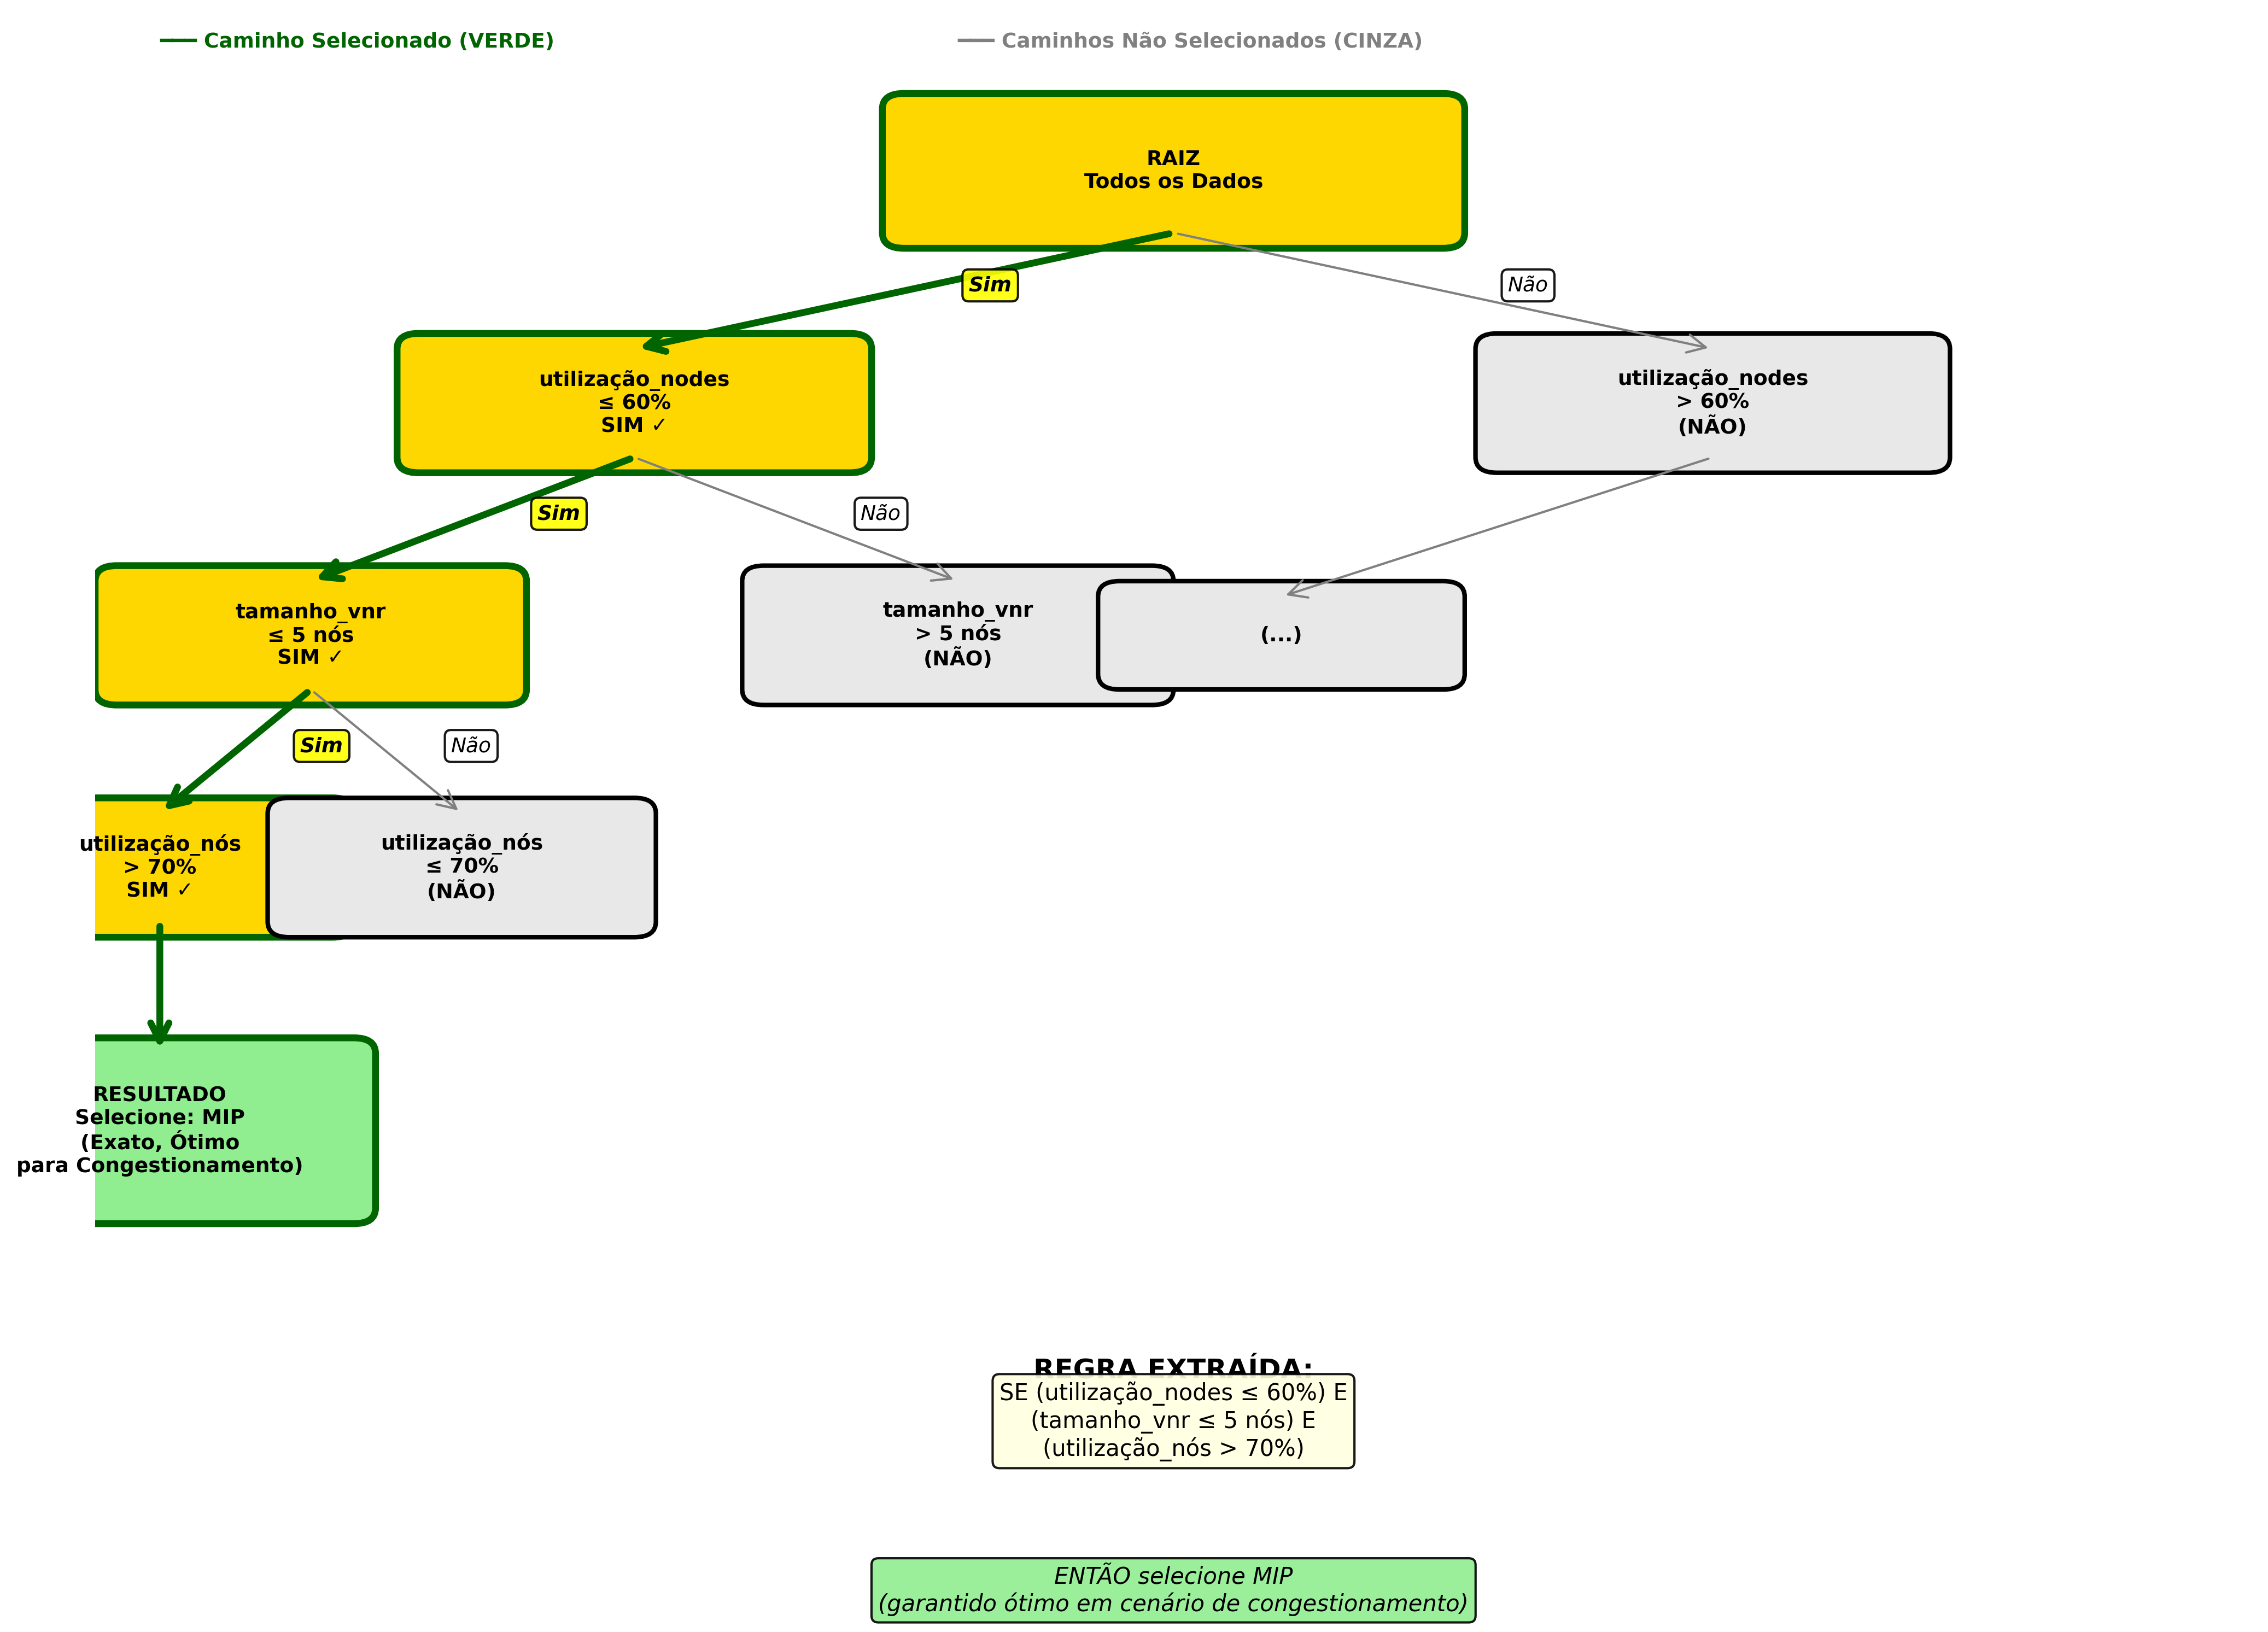
\includegraphics[width=0.95\textwidth]{tree_example_path}
    \caption{Example decision path (root to leaf) for VNE algorithm selection, generated from the trained RAC model on the Fat-Tree topology. The highlighted path leads to the recommendation of MIP under low overall utilization combined with a small, congestion-prone request. Source: authors' own model, trained on the simulation data described in Section~\ref{sec:Proposal}.}
    \label{fig:tree-example-path}
\end{figure}

Unlike deep neural networks or \textit{reinforcement learning} models, each step is comprehensible and auditable by human operators.
Decision trees are particularly suitable for the VNE algorithm selection problem due to the following characteristics:

\begin{itemize}
    \item \textbf{Interpretability}: Each decision can be traced through an explicit logical path in the tree.
    \item \textbf{Robustness to Feature Scale}: Because splits are based on individual feature thresholds rather than distances (as in k-NN or SVM with RBF kernels), decision trees do not require feature normalization, allowing \textit{features} measured in heterogeneous units (e.g., CPU in cores, utilization in percentage) to be combined directly without preprocessing. \textcolor{red}{sera?} \textcolor{red}{[R: a afirmacao e correta para arvores em geral (\emph{splits} univariados por limiar sao invariantes a transformacoes monotonicas), mas esta \textbf{sem referencia} --- viola a diretriz \#8. Vale registrar tambem que, neste trabalho, a heterogeneidade de escala nao e apenas teorica e nao foi tratada: \texttt{resource\_efficiency} tem ordem $10^2$--$10^3$ (\texttt{2\_prepare\_dataset.py:451}) e \texttt{p\_net\_health\_score} chega a $\sim$170 apesar do proprio comentario no codigo documenta-la como ``0-1'' (\texttt{2b\_create\_enhanced\_datasets.py:45-49}).]}
    \item \textbf{Low Latency}: Inference complexity is $O(\text{depth})$. In our experiments (Section~\ref{sec:Results}) prediction latency remained consistently below 1\,ms across all three objectives; this depends on the trained tree depth and the inference hardware, and should not be read as a universal guarantee for arbitrarily deep trees. \textcolor{red}{sempre?} \textcolor{red}{[R: nao, e o texto ja ressalva isso corretamente. A medicao, porem, sustenta ainda menos que o afirmado: o \emph{benchmark} usa \emph{features} aleatorias (\texttt{np.random.rand}, \texttt{benchmark\_inference\_latency.py:46}) e um conjunto de modelos diferente do reportado no restante do artigo. A latencia medida e valida como ordem de grandeza, nao como garantia operacional.]}
    \item \textbf{Explainability}: Operators understand exactly which \textit{features} determined the decision.
\end{itemize}


\subsection{Multi-Objective Optimization}
\label{subsec:multiobj}

The selection of which algorithm to use should not consider only a single performance metric. In real production environments, multiple objectives compete simultaneously: VNR acceptance rate, resolution time, and resource consumption. Approaches that optimize a single objective frequently neglect others, causing system imbalance. The proposed strategy employs multiple specialized trees, each optimized for a specific objective, allowing the system to adapt priorities at runtime according to operational requirements.

The following section positions this work in relation to existing literature, analyzing related work in algorithm selection, multi-objective optimization, and network automation.

\section{Related Work}
\label{sec:RelatedWork}

This section positions the work in relation to existing literature in VNE, algorithm selection, and network automation.
Table~\ref{tab:related-work} synthesizes the comparative analysis between related work and the proposed approach.

\subsection{Algorithm Selection}
\label{subsec:alg-selection}

The algorithm selection problem was formalized by Rice~\cite{rice1976algorithm}, who established the conceptual \textit{framework}: given a problem space, a set of algorithms, a descriptive \textit{feature} space, and performance metrics, determine which algorithm is most appropriate for each problem. This \textit{framework} underlies the approach proposed in this work.

Xu et al.~\cite{xu2012satzilla} develop SATzilla, a portfolio-based selector for satisfiability (SAT) problems, showing that dynamic selection produces significant gains over single algorithms. Similarly, Koslowski et al.~\cite{koslowski2025knowledge-based} apply \textit{machine learning} techniques for the adaptive selection of scheduling policies in high-performance computing (HPC) infrastructures, showing that the consolidation of multiple strategies offers superior adaptability. This paradigm applies equally to the VNE domain. The next subsection discusses how multi-objective optimization has been addressed in related work on virtualized networks.

\subsection{Multi-Objective Optimization in Networks}
\label{subsec:multiobj-networks}

The operational realities of modern networks require simultaneous optimization of multiple objectives: acceptance rate, revenue-cost ratio, average revenue, and processing time. Classical approaches in VNE typically optimize a single objective, neglecting \textit{trade-offs} with others.

Song et al.~\cite{song2020multiobjective} and Belgacem et al.~\cite{belgacem2016multiobjective} explore multi-objective optimization for VNE and resource allocation in virtualized networks, frequently using evolutionary algorithms or dynamic integer programming, which suffer from computational complexity during \textit{online} operation. A detailed positioning of the present approach against this line of work, including the use of independent per-objective models, is presented in the comparative discussion of Section~\ref{subsec:discussion}. \textcolor{red}{precisa disso?} \textcolor{red}{[R: nao ha dado no repositorio a consultar --- e decisao editorial. Trata-se de redundancia estrutural: o mesmo argumento (substituir otimizacao por requisicao por tres modelos sub-milissegundo) ja aparece integralmente na Secao~\ref{subsec:discussion}. A remissao antecipada nao acrescenta conteudo e a subsecao ficaria melhor encerrada por uma ligacao para a proxima (diretriz \#12), nao por um adiamento.]}

\subsection{\textit{Machine Learning} and Reinforcement Learning in Networks}
\label{subsec:ml-networks}

\textit{Machine learning} has become an important tool for network automation.
Cao et al.~\cite{cao2018nfv-deeprl} apply \textit{Deep Reinforcement Learning} (DRL) for dynamic resource allocation in NFV (\textit{Network Function Virtualization}).
Wang et al.~\cite{ijcai-2024-flagvne} propose FlagVNE, a flexible RL \textit{framework} for VNE with multiple policies.

Although DRL offers adaptability, it faces critical challenges for production: long training time (millions of episodes for convergence), lack of interpretability (decisions function as ``black box''), unstable convergence in dynamic environments, and high inference latency (inadequate for real-time decisions).
Recent work on autonomous network systems recognizes that interpretability is a critical requirement for regulated environments~\cite{white2024zerotough}. The next subsection discusses related work specifically on \textit{zero-touch} automation.

\subsection{\textit{Zero-Touch} Automation}
\label{subsec:zerotouchj}

The concept of \textit{Zero-Touch Network and Service Management} (ZSM) was formalized by ETSI since 2017, referring to the operation of network systems with minimal human intervention, through programmable control, virtualization, and closed-loop feedback.

Industry research indicates that reducing manual intervention can decrease operational costs by up to 40\%.
However, the gap between research and production remains: RL systems achieve high performance, but lack adequate interpretability for critical operations.

RSCAT~\cite{diel2023rscat} proposes \textit{zero-touch} automation for congestion control in networks using \textit{actor-critic} reinforcement learning and SDN.
RSCAT shows that combining \textit{machine learning} and classical techniques can enable autonomous operation, similarly to the approach proposed in this work for contextual selection of VNE algorithms. The following subsection synthesizes the comparative analysis between related work and the proposed approach.

\subsection{Discussion}
\label{subsec:discussion}

Table~\ref{tab:related-work} synthesizes a comparative analysis between related work and the proposed approach according to six critical dimensions for production systems:

% NOTA: em coluna unica (LNCS) esta tabela nao cabe na largura do texto.
% O resizebox reduz para caber; alternativas: girar com \rotatebox ou quebrar em duas tabelas.
\begin{table}[t]
\centering
\caption{Comparative Analysis: Related Work vs Proposed Approach (six critical dimensions)}
\label{tab:related-work}
\resizebox{\textwidth}{!}{%
\begin{tabular}{lcccccc}
\toprule
\textbf{Work} & \textbf{ML Type} & \textbf{Adaptive} & \textbf{Multi-Obj.} & \textbf{Interpret.} & \textbf{Latency} & \textbf{Production} \\
\midrule
Fischer (VNE Survey) & Comparison & No & No & Yes & -- & No \\
Rice (Portfolio) & Algorithm & Yes & No & Yes & -- & Conceptual \\
SATzilla & Trees & Yes & No & Yes & Low & Yes \\
Cao et al. (DRL) & Deep RL & Yes & No & No & High (50ms+) & No \\
FlagVNE (DRL) & Deep RL & Yes & No & No & Very High (100ms+) & No \\
\midrule
\textbf{This Work} & \textbf{Multi-Obj. Trees} & \textbf{Yes} & \textbf{Yes (3)} & \textbf{Yes} & \textbf{Very Low $<$1ms} & \textbf{Yes} \\
\bottomrule
\end{tabular}%
}
\end{table}

This work differentiates itself by combining established concepts---algorithm selection, decision trees, and multi-objective optimization---applied to VNE to create a practical and operational solution. Relative to Song et al.~\cite{song2020multiobjective} and Belgacem et al.~\cite{belgacem2016multiobjective}, in particular, the proposed approach replaces per-request evolutionary or integer-programming optimization with three independently trained, sub-millisecond decision-tree models, letting an operator select at runtime which objective (RAC, LRC, or LAR) to prioritize without re-solving an optimization problem online. The main distinctive contributions include:
\begin{itemize}
    \item \textbf{Multi-Objectivity}: Three specialized models, not just acceptance optimization. Operators can adapt priorities at runtime as operational conditions change.

    \item \textbf{Contextual Adaptability}: Selection based on real network state (utilization, fragmentation) and request characteristics (size, connectivity), not just VNR characteristics.

    \item \textbf{Complete Interpretability}: Unlike RL/DL approaches (black box), each decision can be explained to operators through explicit paths in the decision tree.

    \item \textbf{Computational Efficiency}: Training in seconds (not millions of episodes), inference in sub-milliseconds ($<$1ms), enabling real-time \textit{online} operation.

    \item \textbf{Practical Validation}: Presents a real improvement in acceptance rate of +38.78 percentage points (from 43.17\% to 81.95\%, +89.83\% relative) in a realistic simulated environment with 8,000 virtual network requests across three topologies, together with gains of +58.76\% in revenue-cost ratio and +61.40\% in average revenue (see Section~\ref{sec:Results}).
\end{itemize}

The following section details the proposed methodology, describing the steps of data collection, \textit{feature} engineering, model training, and \textit{online} prediction.

\section{Methodology}
\label{sec:Proposal}

\subsection{Approach Overview}

The methodology consists of four main steps:

\begin{enumerate}
    \item \textbf{Data Collection}: Execute eight VNE algorithms---\textit{MIP, GA-Meta, PSO-Meta, SA-Meta, MCTS, PL-Rank, RW-Rank-BFS, D-Round}---on three distinct topologies---\textit{Tree, Fat-Tree (k=4) and Waxman-16}---and collect detailed performance data in each scenario for model training, validation, and testing.
    \item \textbf{Feature Engineering}: Extract 27 relevant characteristics from VNRs, network state, and topological context.
    \item \textbf{Multi-Objective Training}: Create three specialized models---RAC (\textit{Request Acceptance Rate}), LRC (\textit{Long-term Revenue-to-Cost Ratio}) and LAR (\textit{Long-term Average Revenue})---, each optimizing specific performance criteria.
    \item \textbf{Online Prediction}: For each new VNR, use the extracted context to dynamically select the most appropriate VNE algorithm through the model that optimizes the desired criterion.
\end{enumerate}

\subsection{Simulation Data Generation}

Data were collected using the \textbf{Virne}~\cite{wang2024virne} platform, a comprehensive \textit{benchmarking} \textit{framework} for Network Function Virtualization Resource Allocation (NFV-RA) problems. Virne offers highly customizable simulations for various network scenarios, including cloud \textit{datacenters}, edge computing, and 5G networks. The platform implements more than 30 NFV-RA algorithms in a modular and extensible architecture, providing an \textit{event-driven} simulation environment that models the physical network (PN) infrastructure and sequential virtual network requests (VNRs). Each VNR arrival is treated as a discrete event, creating an instance that the NFV-RA algorithm must solve, evaluating solution feasibility and updating network resources.

Simulations were executed with eight VNE algorithms on three distinct topologies, commonly used in \textit{datacenters}:

\medskip
\noindent\textbf{Topologies}:
\begin{itemize}
    \item \textbf{Tree}: A binary tree with 32 hosts and 31 switches (63 nodes)
    \item \textbf{Fat-Tree}: \textit{Datacenter} with k=4 (16 servers, 20 switches, 36 nodes)
    \item \textbf{Waxman-16}: Random network with 16 nodes and 500 links \textcolor{red}{[R: impossivel --- um grafo simples nao-direcionado de 16 nos admite no maximo $16 \times 15 / 2 = 120$ enlaces. Verificar o valor real gerado pelo Virne para os parametros $\alpha$=0,5 e $\beta$=0,2 citados na legenda da Figura~\ref{fig:waxman-topology}.]}
\end{itemize}

Figure~\ref{fig:topologies-comparison} presents visualization of the Tree and Fat-Tree topologies used in the simulations, showing their distinct hierarchical structures:

\begin{figure}[htbp]
    \centering
    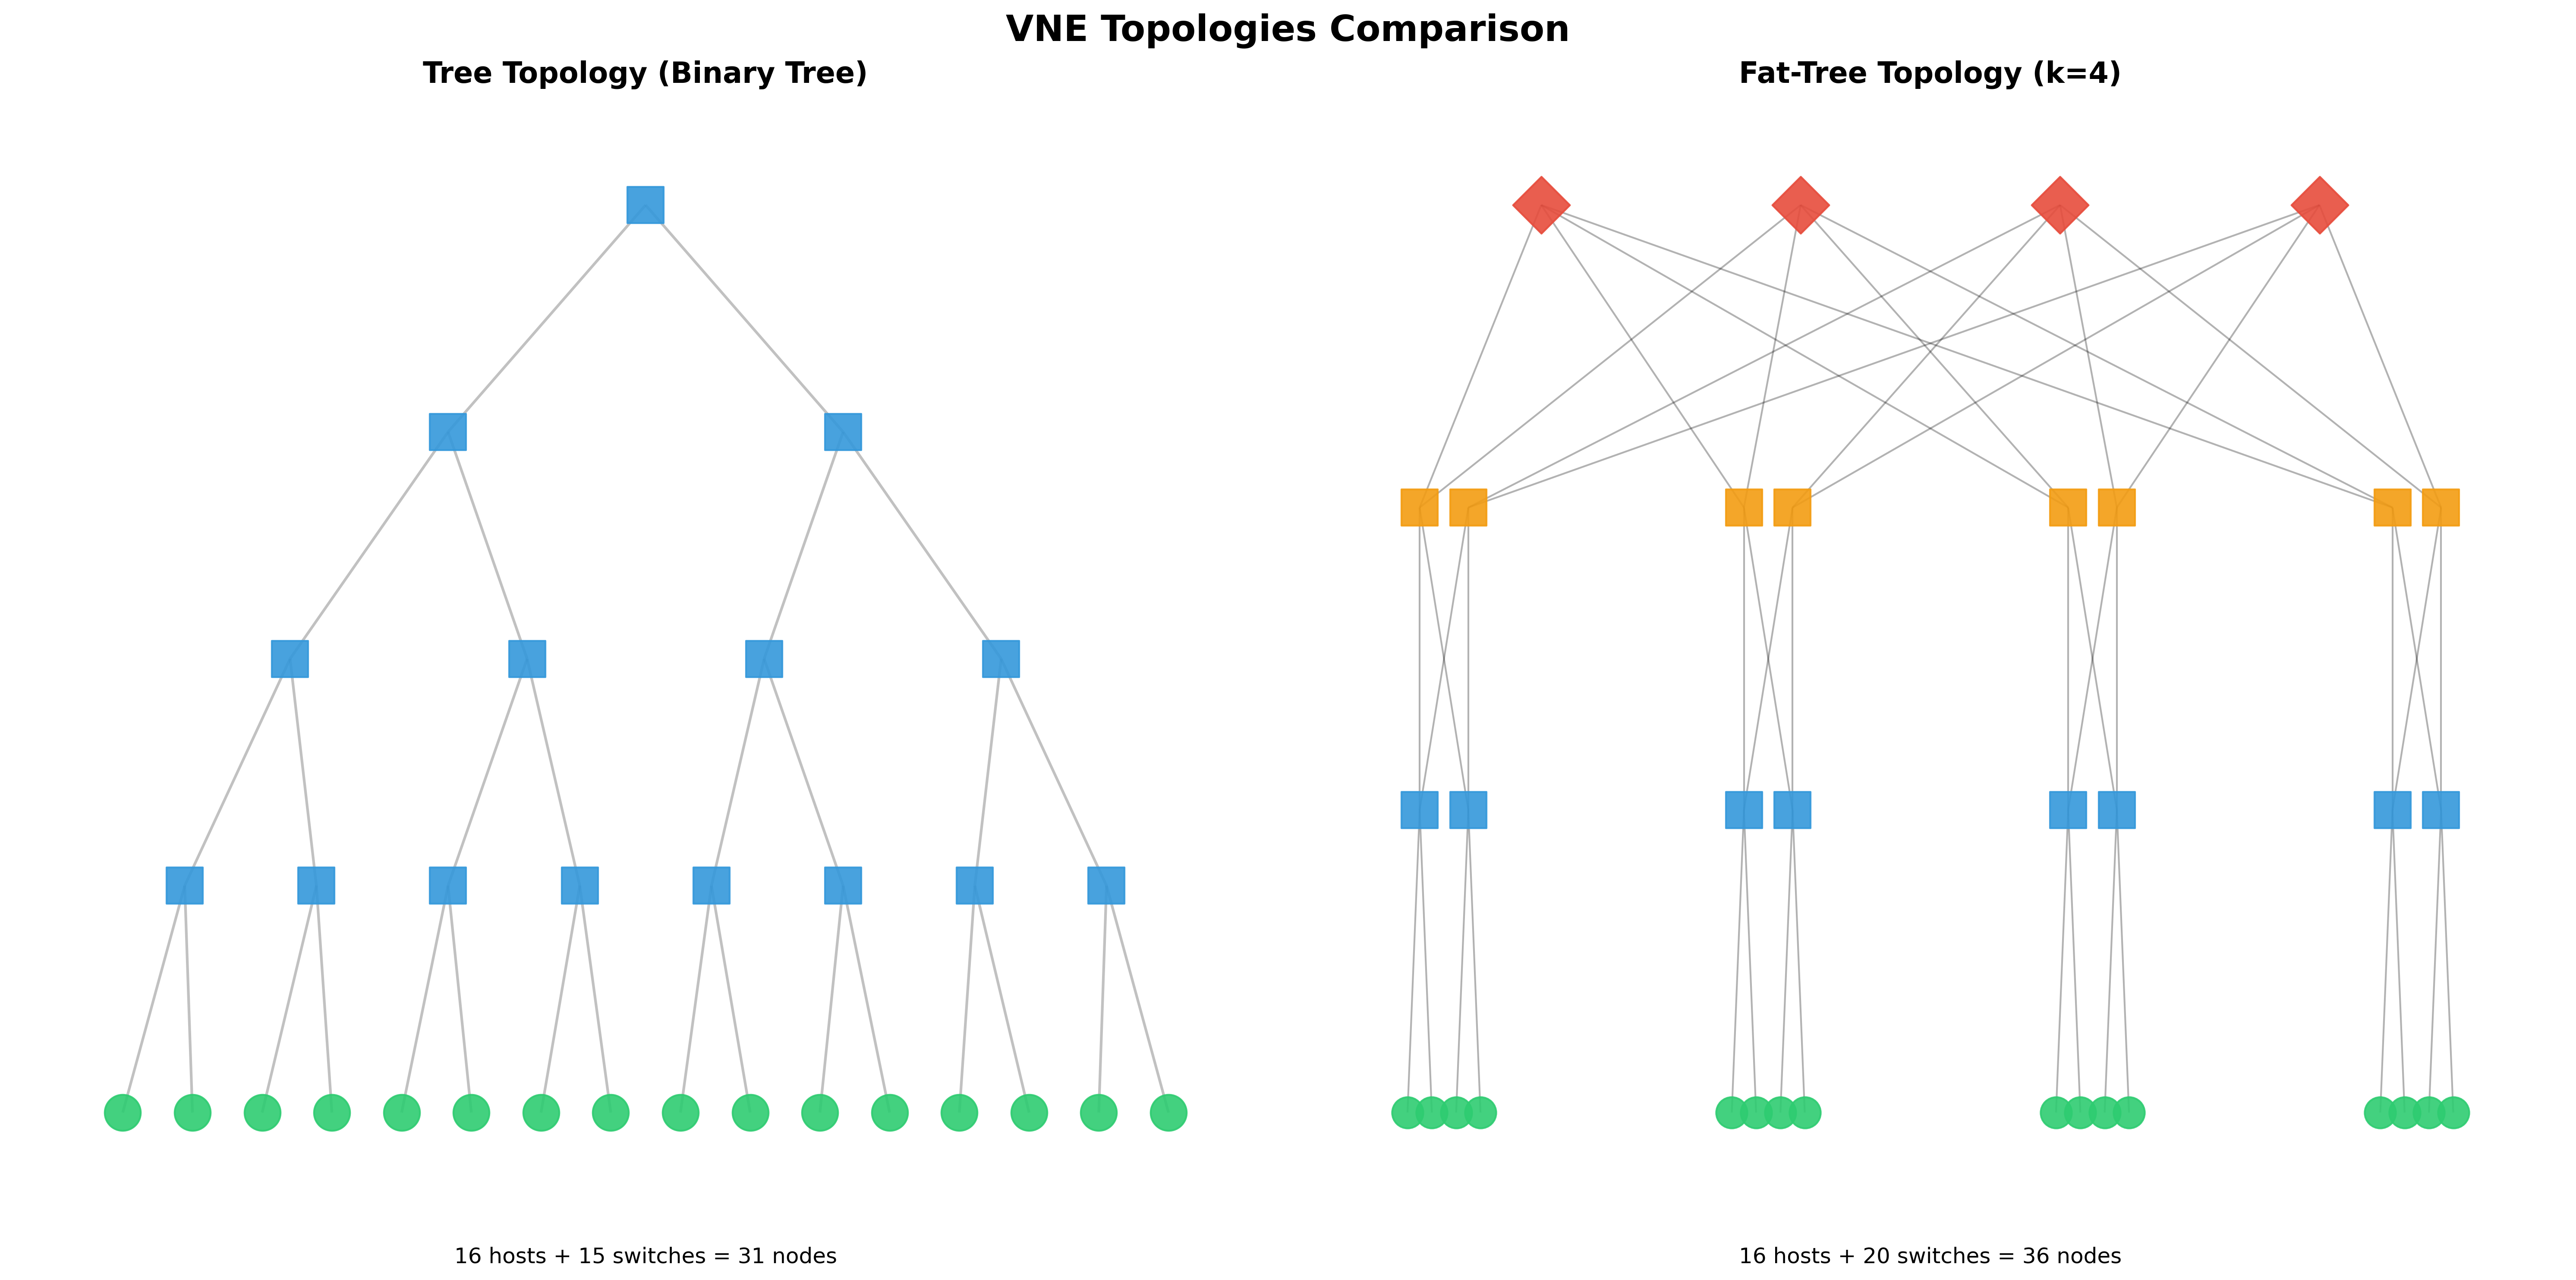
\includegraphics[width=0.95\textwidth]{topologies_comparison}
    \caption{Topology Comparison: Tree (Binary Hierarchical) and Fat-Tree (\textit{Datacenter}). The Tree topology presents a traditional hierarchical structure with hosts at the base and switches at successive levels. The Fat-Tree presents a \textit{datacenter} structure with k=4, characterized by multiple paths and greater redundancy.}
    \label{fig:topologies-comparison}
\end{figure}

Figure~\ref{fig:waxman-topology} presents the third topology used in the simulations, Waxman-16, which represents a random network with characteristics distinct from the previous structured topologies:

\begin{figure}[htbp]
    \centering
    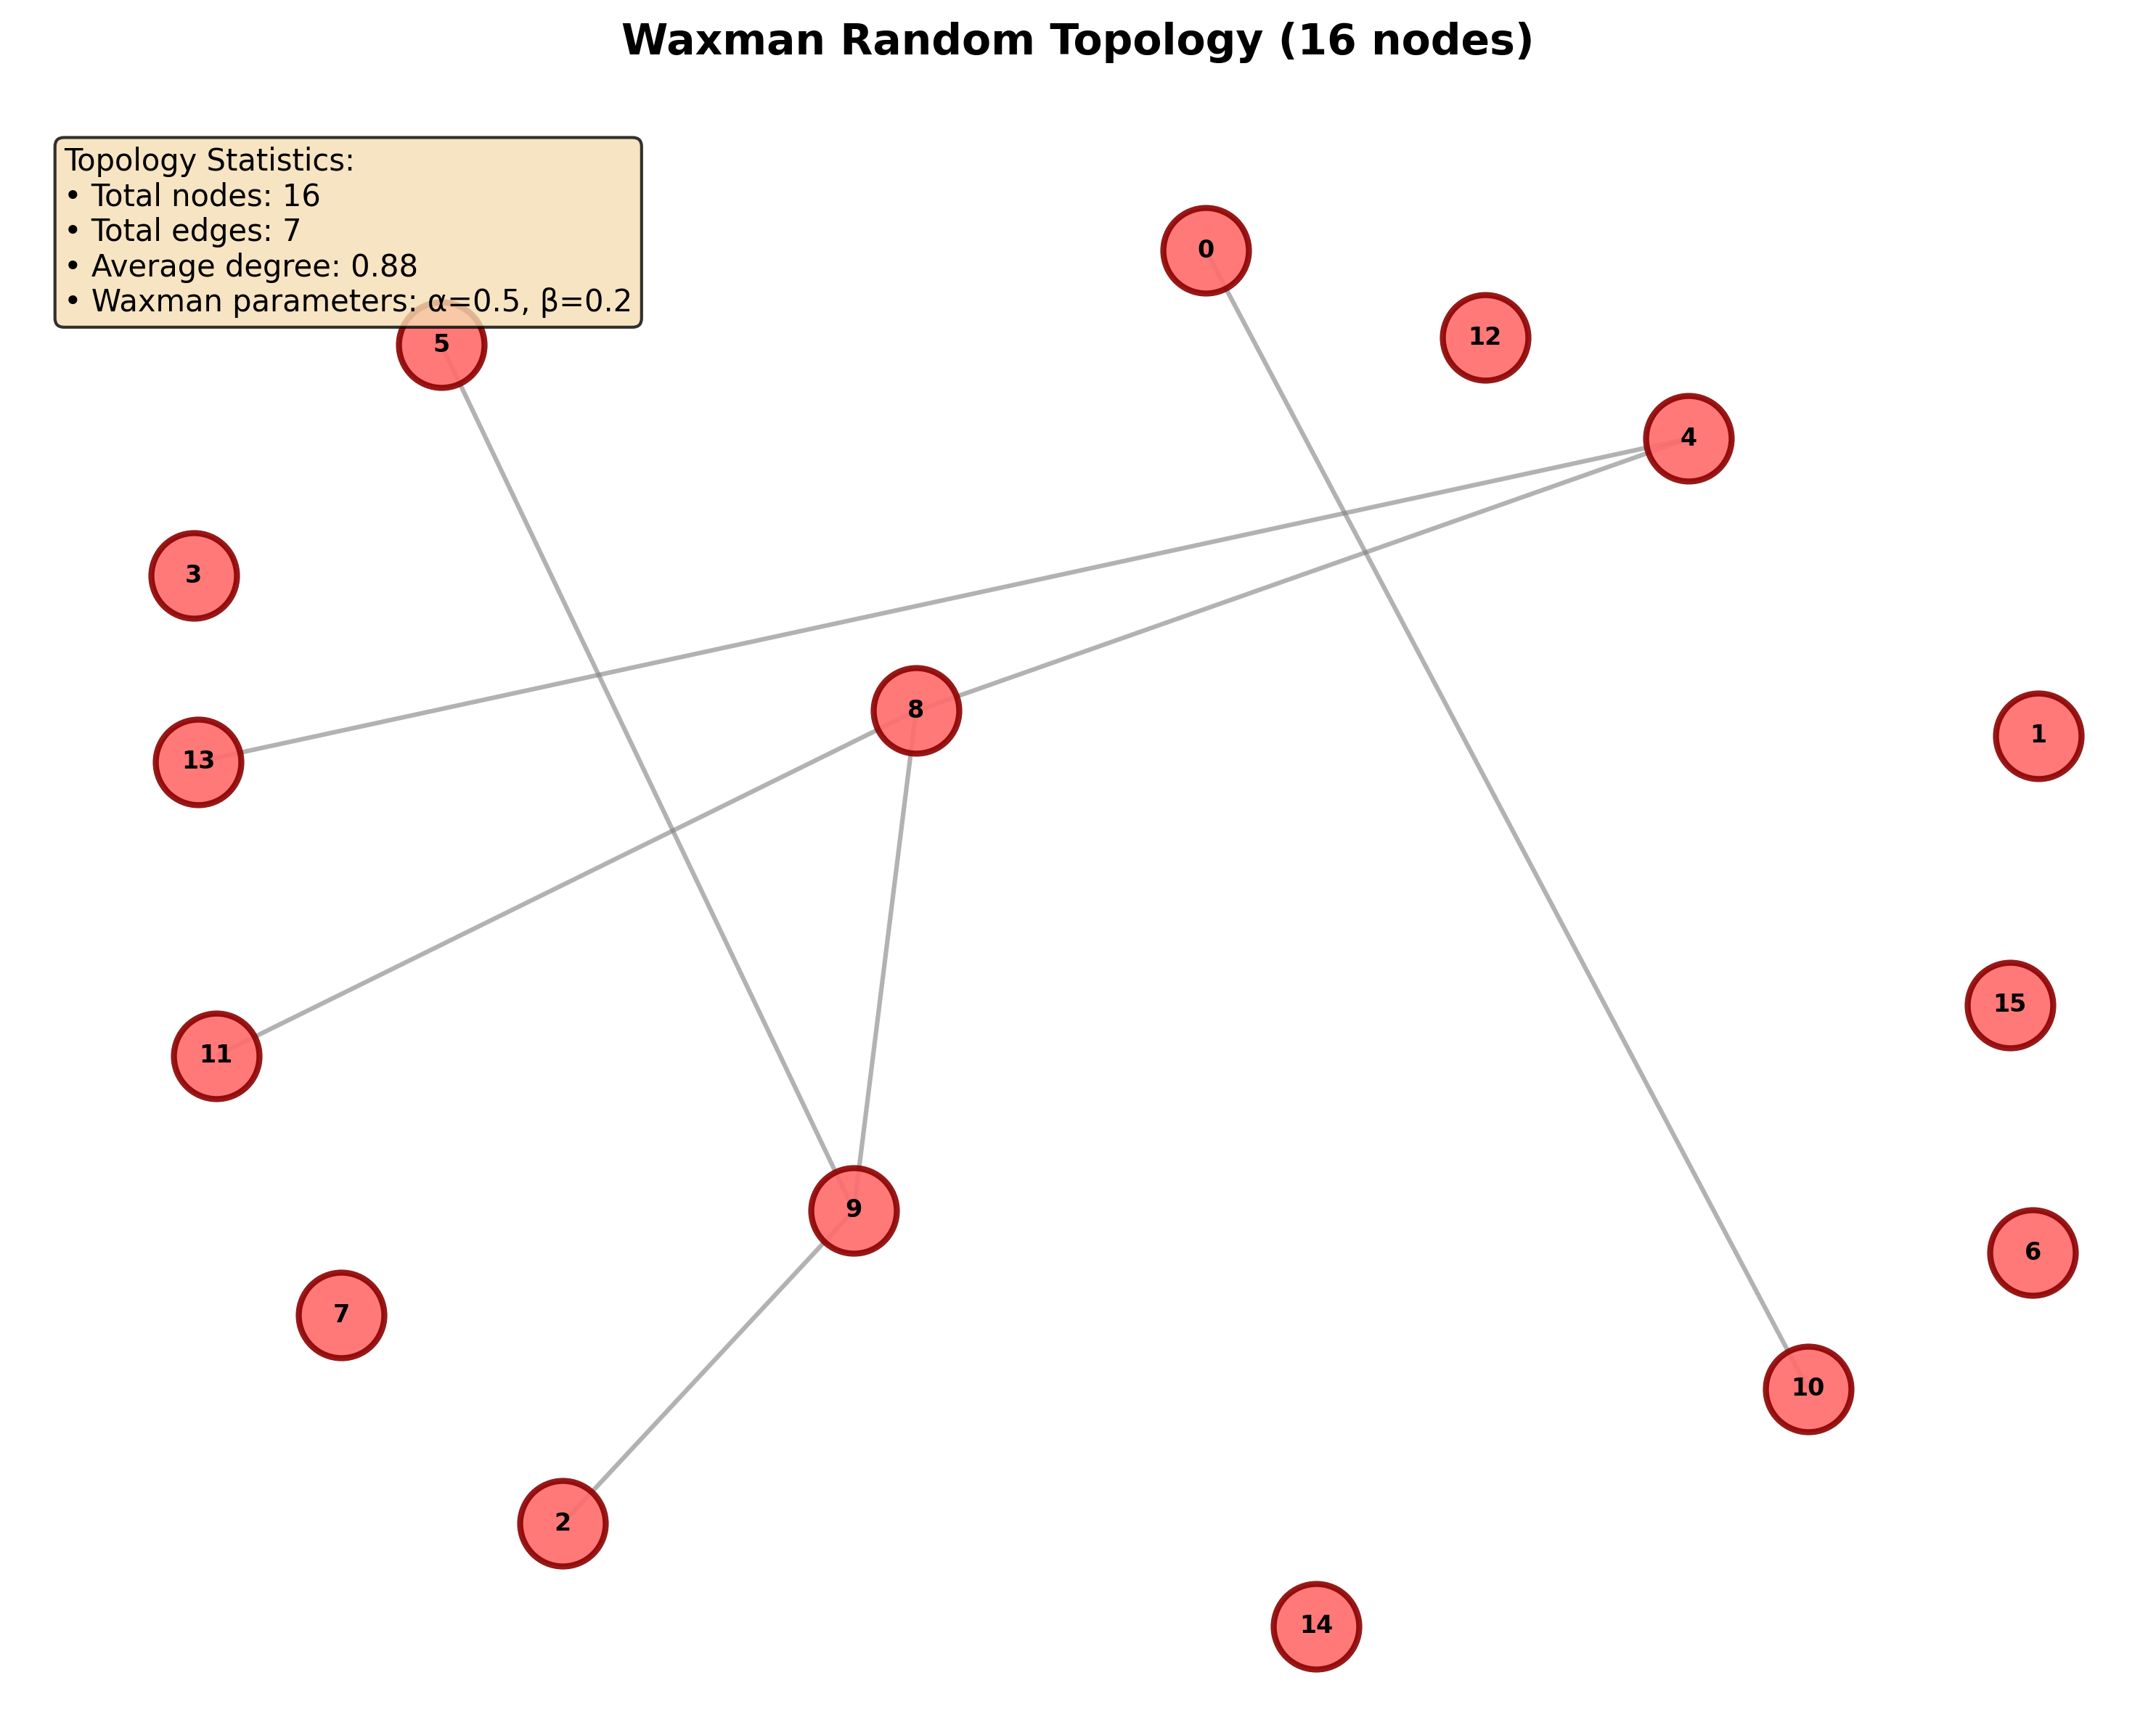
\includegraphics[width=0.7\textwidth]{waxman_16_topology}
    \caption{Waxman-16 Topology: Random Network with 16 Nodes. Unlike structured topologies (Tree and Fat-Tree), Waxman represents a random network generated with geographic dispersion parameters ($\alpha$=0.5, $\beta$=0.2), simulating characteristics of real large-scale networks, with multiple isolated nodes and variable connected groups.}
    \label{fig:waxman-topology}
\end{figure}

\noindent\textbf{VNE Algorithms}: MIP, GA-Meta, PSO-Meta, SA-Meta, MCTS, PL-Rank, RW-Rank-BFS, D-Round.

\medskip
Simulations were configured with homogeneous resources (CPU and memory) uniformly distributed on physical nodes. VNRs were generated with variable size (uniform distribution between 2 and 10 virtual nodes), 50\% connectivity between virtual nodes, and resource demands following realistic distributions. The system simulates sequential VNR arrivals with arrival rate according to Poisson distribution, where each request has a stochastic lifetime. Virne automatically evaluates the feasibility of each solution proposed by the algorithms, verifying node and link capacity constraints, and calculates standardized performance metrics (RAC, LRC, LAR, AST) for each execution.

For each combination of algorithm and topology, ten repetitions were executed with different random seeds, totaling approximately 8,000 unique VNRs after deduplication. \textcolor{red}{[R: nenhum dos dois numeros confere com os dados. As sementes efetivamente presentes sao \textbf{cinco} (0 a 4), nao dez, e \texttt{datasets/vnr\_clean.csv} contem \textbf{4.500} VNRs unicas (1.500 por topologia), nao 8.000. Alem disso, a ``deduplicacao'' e apenas um \texttt{.first()} arbitrario (\texttt{2\_prepare\_dataset.py:203,480}) sobre $\sim$4,7 registros conflitantes por grupo --- ver anotacao detalhada na Secao~\ref{sec:Results}. Note ainda que o numero 8.000 reaparece na Secao de latencia, onde o valor real do codigo e 10.000 iteracoes.]} This approach ensures statistical robustness and captures the variability inherent to stochastic algorithms and dynamic characteristics of virtual network requests.

\textcolor{red}{[: explicitar aqui a baseline]}

\textcolor{red}{[R: a \emph{baseline} implementada e a \textbf{classe majoritaria do rotulo} no conjunto de teste --- isto e, ``prever sempre o algoritmo mais frequentemente rotulado como otimo'' --- e \textbf{nao} o algoritmo de melhor desempenho medio, como a leitura do texto sugere. Definicao em \texttt{5\_evaluate\_performance\_improvement.py:217-230} (\texttt{calculate\_baseline\_algorithm}): \texttt{algo\_counts = test\_df[label\_col].value\_counts()}, \texttt{baseline\_algo = algo\_counts.index[0]}. Concretamente: \texttt{ga\_meta} para RAC e LAR, \texttt{pl\_rank} para LRC.
Observacao relevante: o mesmo arquivo define tambem um \texttt{best\_global\_algorithm} (linhas 233-245), que para RAC resulta em \texttt{mip} com 32,93\% --- \emph{pior} que os 43,17\% da \emph{baseline} reportada. Esse numero nao aparece no artigo. Se um revisor perguntar ``por que nao comparar com o melhor algoritmo fixo?'', a resposta atual do codigo e desfavoravel e precisa ser explicitada.]}

\subsection{Feature Engineering}

A set of 27 features was carefully selected, divided into categories:

\medskip
\noindent\textbf{VNR Characteristics} (9 features): number of nodes, number of links, size ratio, average demand per node, average demand per link, connectivity, total demand, node/link ratio, expected lifetime.

\noindent\textbf{Physical Network State} (4 features): available resources, node utilization, link utilization, overall utilization.

\noindent\textbf{System State} (3 features): number of active VNRs, system load, active physical nodes.

\noindent\textbf{Heterogeneity and Fragmentation} (10 engineered features): Gini indices for resource distribution, memory fragmentation, topological diversity indices.

\noindent\textbf{Context} (1 feature): topology type.

\subsection{Multi-Objective Architecture}

Instead of a single classification model, we employ \textbf{three specialized models}, each optimized for a specific objective:

\begin{itemize}
    \item \textbf{RAC}: Maximize virtual network request acceptance rate
    \item \textbf{LRC}: Maximize long-term revenue-cost ratio
    \item \textbf{LAR}: Maximize long-term average revenue
\end{itemize}

Each model is a decision tree trained independently on the same 27 input features described above, but with a different target label: for a given VNR, the label used to train the RAC model is the algorithm (among the eight candidates) that achieved the best acceptance outcome for that request in the simulation data, while the LRC and LAR models use the algorithm that achieved the best revenue-cost ratio and average revenue, respectively. This produces three independent classifiers that share the same input representation but learn different notions of ``best algorithm.''

During \textit{online} operation, the network operator (or an automatic control policy) specifies which objective currently has priority --- for example, favoring acceptance rate during periods of high demand, or favoring revenue-cost ratio when profitability is the primary concern. The corresponding model (RAC, LRC, or LAR) is then queried with the current physical network state and the incoming VNR's features, and returns the algorithm predicted to perform best for that objective under the current conditions. Consequently, the same VNR can receive different algorithm recommendations depending on which of the three objectives is active at decision time. \textcolor{red}{nao entendi direito} \textcolor{red}{[R: o mecanismo descrito confere com o codigo (tres \texttt{DecisionTreeClassifier} independentes, mesma matriz de entrada, rotulos \texttt{best\_for\_rac}/\texttt{best\_for\_lrc}/\texttt{best\_for\_lar} distintos --- ver \texttt{3\_train\_decision\_trees\_balanced.py}). O que falta ao texto sao dois elementos concretos: (i) \emph{quem} define o objetivo ativo e em que momento (nao ha politica de chaveamento implementada --- o objetivo e um parametro escolhido manualmente na chamada de inferencia); e (ii) um exemplo numerico de uma mesma VNR recebendo recomendacoes diferentes conforme o objetivo, que tornaria a ideia imediatamente compreensivel (diretriz \#6).]}

\subsection{Model Training}

The training process was performed independently for each objective (RAC, LRC, LAR), allowing each model to specialize in optimizing its specific metric. Data division was stratified by algorithm class to ensure balanced distribution between training (70\%), validation (15\%), and test (15\%) sets. This stratification helps maintain representativeness of all classes in each partition, especially considering the severe imbalance observed in the data.

Models use \texttt{DecisionTreeClassifier} from scikit-learn~\cite{pedregosa2011scikit-learn}\textcolor{red}{fonte} \textcolor{red}{[R: a citacao \texttt{pedregosa2011scikit-learn} existe e esta correta em \texttt{references.bib}. Duas lacunas provaveis por tras da marcacao: (i) a \textbf{versao} da biblioteca nao esta registrada em nenhum script nem em arquivo de ambiente, o que compromete a reprodutibilidade; e (ii) os hiperparametros abaixo sao apresentados como ``optimized'' mas nao ha referencia nem procedimento de busca documentado --- estao fixos em \texttt{3\_train\_decision\_trees\_balanced.py:378-380} (\texttt{max\_depth=10}, \texttt{min\_samples\_leaf=3}, \texttt{min\_samples\_split=6}). Ou se referencia o metodo de escolha, ou se remove o adjetivo ``optimized'' (diretriz \#27).]} with the following optimized hyperparameters:

\begin{itemize}
    \item \textbf{Maximum depth}: 10 (balancing expressiveness and interpretability)
    \item \textbf{Minimum samples per leaf}: 3 (reduced to allow capture of minority classes)
    \item \textbf{Minimum samples for split}: 6 (allows splits with fewer samples)
    \item \textbf{Splitting criterion}: Gini (Gini impurity for \textit{feature} selection)
\end{itemize}

\textcolor{red}{[R: atencao --- os valores da Tabela~\ref{tab:algorithm-summary} nao sao medidos, sao \emph{proxies} calculadas (\texttt{12\_algorithm\_comparison\_metrics.py:38-66}): receita $=$ \texttt{n\_aceitos} $\times$ (150 $-$ \texttt{lar}); razao receita/custo $=$ \texttt{aceitacao} / \texttt{lrc}; tempo $=$ \texttt{lar} / 100. Nenhuma das tres colunas corresponde a uma grandeza observada na simulacao. Ha ainda um problema de denominador: as taxas de aceitacao usam contagens de registros diferentes por algoritmo (\texttt{mip} 10.687 contra \texttt{ga\_meta} 16.000), o que e o que faz \texttt{mip} aparecer em primeiro lugar. Nos dados brutos por VNR a ordem real de aceitacao e \texttt{pl\_rank} 48,8\% $>$ \texttt{ga\_meta} 37,5\% $>$ \texttt{sa\_meta} 36,5\% $>$ \texttt{mcts} 36,0\% $>$ \texttt{mip} 29,6\% --- ou seja, a afirmacao ``MIP maximizes acceptance rate'', repetida na Secao~\ref{sec:Results}, esta invertida. A conclusao qualitativa (nenhum algoritmo domina) permanece valida, mas precisa ser sustentada por metricas medidas.]}

As shown in Table~\ref{tab:algorithm-summary}, no algorithm is universally optimal, evidencing the need for contextual selection. This observation justifies the dynamic algorithm selection approach proposed in this work.

\begin{table}[htbp]
\centering
\caption{VNE Algorithm Performance Summary (values are simulation-native metric units, not currency; revenue is reported per topology-algorithm combination, aggregated over all seeds).}
\label{tab:algorithm-summary}
\begin{tabular}{lcccc}
\toprule
\textbf{Algorithm} & \textbf{Acceptance Rate} & \textbf{Revenue} & \textbf{R2C Ratio} & \textbf{Time (s)} \\
\midrule
MIP & 36.8\% & 186.8 & 115.6 & 1.026 \\
PL\_RANK & 29.5\% & 388.4 & 127.4 & 0.661 \\
GA\_META & 27.9\% & 400.6 & 139.8 & 0.603 \\
RW\_RANK\_BFS & 25.8\% & 373.9 & 120.4 & 0.558 \\
SA\_META & 24.6\% & 372.6 & 133.5 & 0.534 \\
MCTS & 23.9\% & 379.7 & 167.0 & 0.468 \\
D\_ROUND & 20.4\% & 365.4 & 246.0 & 0.357 \\
PSO\_META & 20.1\% & 352.1 & 120.0 & 0.309 \\
\bottomrule
\end{tabular}
\end{table}

\subsection{Multi-Metric Comparison of VNE Algorithms}

VNE algorithm selection cannot be based on a single performance metric. Different operational contexts (high load, limited resources, latency requirements) require different \textit{trade-offs}. Figure~\ref{fig:algorithm-comparison} presents a comprehensive analysis of four complementary metrics for the eight evaluated algorithms:

\begin{figure}[htbp]
    \centering
    \includegraphics[width=\textwidth]{algorithm_comparison_all_metrics}
    \caption{Multi-Metric Comparison: Acceptance Rate, Total Revenue, Revenue-Cost Ratio, and Average Time per VNR. Each panel shows the distribution of results across ten random-seed repetitions per algorithm and topology (Tree, Fat-Tree, Waxman-16). No single algorithm is optimal in all four dimensions. Source: authors' own simulation results (Section~\ref{sec:Proposal}).}
    \label{fig:algorithm-comparison}
\end{figure}

\subsubsection{Class Balancing Techniques.}

To reduce dataset imbalance, class balancing techniques were applied:

\medskip
\noindent\textbf{Custom Class Weights}: Instead of scikit-learn's default balancing, weights calculated as $w_i = 1/\sqrt{f_i}$ were used, where $f_i$ is the relative frequency of class $i$. This strategy assigns significantly larger weights to rare classes:

\begin{itemize}
    \item Rare classes (\texttt{pso\_meta}, 17 samples): weight 10.0$\times$
    \item Intermediate classes (\texttt{rw\_rank\_bfs}, 39 samples): weight 6.6$\times$
    \item Majority classes (\texttt{ga\_meta}, 987 samples): weight 1.3$\times$
\end{itemize}

\noindent\textbf{Evaluation}: Performance is evaluated per class using precision, recall, and F1-Score. Two aggregate metrics are also reported: \emph{F1-Weighted} (the F1-Score of each class weighted by its support, favoring frequent classes) and \emph{F1-Macro} (the unweighted arithmetic mean of per-class F1-Scores, treating all classes---including rare ones---equally). Reporting both metrics together makes the impact of class imbalance on the balanced model explicit.

\subsection{Detailed F1-Score Analysis per Class}
\textcolor{red}{como foi calculado? baseline ta ruimm}

\textcolor{red}{[R: a preocupacao procede --- esta e a anotacao de maior risco do artigo. O rastreamento no codigo revelou cinco pontos, todos verificados empiricamente:
\textbf{(1) Nao ha re-simulacao.} O ``real operational performance'' e \emph{replay} tabular \emph{offline}: a funcao \texttt{get\_vnr\_result()} (\texttt{5\_evaluate\_performance\_improvement.py:248-284}) apenas consulta linhas ja gravadas em \texttt{vnr\_raw\_data.csv}. Nada e re-executado no Virne, ou seja, o resultado nao captura o efeito do algoritmo escolhido sobre o estado futuro da rede.
\textbf{(2) A topologia Waxman-16 e descartada silenciosamente.} \texttt{vnr\_raw\_data.csv} contem somente \texttt{tree} e \texttt{fat\_tree}; \texttt{waxman\_16\_raw\_data.csv} nunca e carregado por esse script. O conjunto de teste tem 617 VNRs (tree 186 + fat\_tree 224 + waxman 207), e 186+224 = \textbf{410}, exatamente o valor de \texttt{tree\_matched} em \texttt{balanced\_performance\_improvement.json}. Portanto \textbf{todos} os numeros de desempenho real do artigo vem de 410 VNRs e \textbf{duas} topologias, embora o texto afirme tres.
\textbf{(3) O oraculo RAC = 1,0 e tautologico.} O rotulo \texttt{best\_for\_rac} e, por construcao, um algoritmo que aceitou a requisicao; reproduzi-lo sempre devolve \texttt{success=True}. O ``teto'' de 100\% nao e um resultado, e uma identidade.
\textbf{(4) A chave \texttt{(topology, seed, v\_net\_id)} nao identifica uma VNR.} Em 3.000 de 3.000 grupos, os oito algoritmos supostamente comparados ``sobre a mesma VNR'' apresentam \texttt{v\_net\_demand} diferente; em 2.999/3.000, tambem \texttt{v\_net\_num\_nodes} difere. Ha $\sim$4,7 registros duplicados por grupo, colapsados por um \texttt{.first()} arbitrario (\texttt{2\_prepare\_dataset.py:203}).
\textbf{(5) O rotulo RAC e um desempate alfabetico em 74\% dos casos.} \texttt{accepted.iloc[0]} apos \texttt{groupby('algorithm')} ordena alfabeticamente; em 2.008 de 2.707 VNRs rotuladas ha dois ou mais algoritmos que aceitaram. Isso explica a dominancia de \texttt{ga\_meta} --- que e justamente a \emph{baseline}.
\textbf{Contraponto interno ao repositorio:} o experimento \texttt{ccis/}, que avalia todos os candidatos sobre o \emph{mesmo} estado da rede, obtem arvore 47,0\% contra melhor fixo (\texttt{mip}) 49,3\% (\texttt{ccis/results/tree\_summary.json}, \texttt{gap\_captured: -0.933}). O proprio \texttt{ccis/README.md:18-31} classifica a rotulagem usada neste artigo como causalmente invalida.]}

Table~\ref{tab:f1-per-class} presents the F1-Score per class for the RAC objective, computed on the held-out test split (15\% of the data, Section~\ref{sec:Proposal}) using the class weights and metrics defined above. Results indicate that even minority classes, such as PSO\_Meta and RW\_Rank\_BFS, present F1-Score above 0.33 after balancing, compared to near-zero recall observed for these classes prior to applying the custom weights.

\section{Experimental Results}
\label{sec:Results}

Unless otherwise noted, all figures and tables in this section present results generated from the authors' own simulation experiments on the Virne platform, described in Section~\ref{sec:Proposal}; no external or third-party data is used.

\subsection{Classification Performance}

Table~\ref{tab:classification-metrics} presents the classification metrics obtained for the three considered objectives (RAC, LRC, and LAR). In addition to standard top-1 accuracy, we report \emph{top-2} and \emph{top-3 accuracy}: the percentage of test instances in which the true best-performing algorithm is included among, respectively, the two or three algorithms the model ranks as most likely. This metric is practically relevant because, operationally, recommending one of the top few near-optimal algorithms is often as useful as recommending the single best one, especially given how close several algorithms' performance can be (Table~\ref{tab:algorithm-summary}).

\begin{table}[htbp]
\centering
\caption{Classification Metrics by Objective (Balanced Models)}
\label{tab:classification-metrics}
\begin{tabular}{lcccc}
\toprule
\textbf{Objective} & \textbf{Accuracy} & \textbf{F1-Score} & \textbf{Top-2} & \textbf{Top-3} \\
\midrule
RAC (Acceptance Rate) & 67.26\% & 0.68 & 82.66\% & 85.90\% \\
LRC (Revenue-Cost Ratio) & 54.46\% & 0.55 & 74.55\% & 83.95\% \\
LAR (Average Revenue) & 48.14\% & 0.48 & 67.59\% & 79.09\% \\
\bottomrule
\end{tabular}
\end{table}

Results presented in Table~\ref{tab:classification-metrics} indicate that the RAC objective presents better performance in all metrics, with top-1 accuracy of 67.26\% and top-3 accuracy of 85.90\% \textcolor{red}{o que é isso} \textcolor{red}{[R: e o percentual de instancias de teste em que o algoritmo verdadeiramente melhor esta entre os tres mais provaveis segundo o modelo. O calculo usa \texttt{top\_k\_accuracy\_score} do scikit-learn sobre \texttt{predict\_proba} (\texttt{4\_evaluate\_trees.py:99-103}), e os valores da Tabela~\ref{tab:classification-metrics} \textbf{reproduzem exatamente} ao recarregar os \texttt{.pkl} e o \texttt{test.csv}.
Duas ressalvas a considerar: (i) a metrica ja e definida no inicio desta subsecao, mas aparece antes disso no resumo (o que provavelmente motivou a marcacao) --- convem antecipar a definicao ou evita-la no resumo; (ii) \texttt{predict\_proba} de uma arvore devolve a frequencia de classes na folha, e com \texttt{min\_samples\_leaf=3} muitas folhas tem tres ou menos amostras, de modo que o ranqueamento top-2/top-3 frequentemente ordena empates de probabilidade zero, desempatados pelo indice da classe. A metrica e valida, mas menos informativa do que aparenta neste regime.]}. The LRC objective presents intermediate performance, while LAR presents lower top-1 accuracy (48.14\%), but still with top-3 accuracy of 79.09\%, indicating that the model frequently identifies the best algorithm among the top three options even when it does not rank it first. The performance difference between objectives reflects the distinct complexity of each metric and the inherent variability of algorithms in different contexts.

\subsection{Comparison with \textit{Baseline}}

This subsection compares two related but distinct quantities: (i) \emph{classification accuracy} at predicting the best algorithm, and (ii) the \emph{real operational performance} obtained when the predicted algorithm is actually used to serve each VNR in simulation. Figure~\ref{fig:baseline-comparison} addresses the first; Figure~\ref{fig:real-performance-improvement} addresses the second.

\begin{figure}[htbp]
\centering

\includegraphics[width=0.95\textwidth]{baseline_comparison_chart}
\caption{Classification Accuracy Comparison: Fixed-Algorithm Baseline vs Decision Tree, by Optimization Objective. Bars show the percentage of test VNRs for which the baseline's fixed choice, versus the decision tree's predicted choice, matches the true best-performing algorithm for that objective. Source: authors' own experimental results.}
\label{fig:baseline-comparison}
\end{figure}

Figure~\ref{fig:baseline-comparison} shows that, in terms of \emph{classification accuracy} (how often the correct best algorithm is identified), the decision tree significantly outperforms always predicting the fixed baseline algorithm. For the RAC objective, the improvement is +32.90 percentage points (+95.8\% relative), while for LRC and LAR the improvements are even more expressive in relative terms (+100.0\% and +110.7\%, respectively).

To validate that these classification gains translate into real operational performance improvement, and not merely into more accurate labels, we evaluated the actual RAC/LRC/LAR values obtained when decision trees are used to select the algorithm executed for each VNR in simulated operation, and compared this to always using the fixed baseline algorithm.
Figure~\ref{fig:real-performance-improvement} presents this comparison of real, per-VNR operational performance.

\begin{figure}[htbp]
\centering
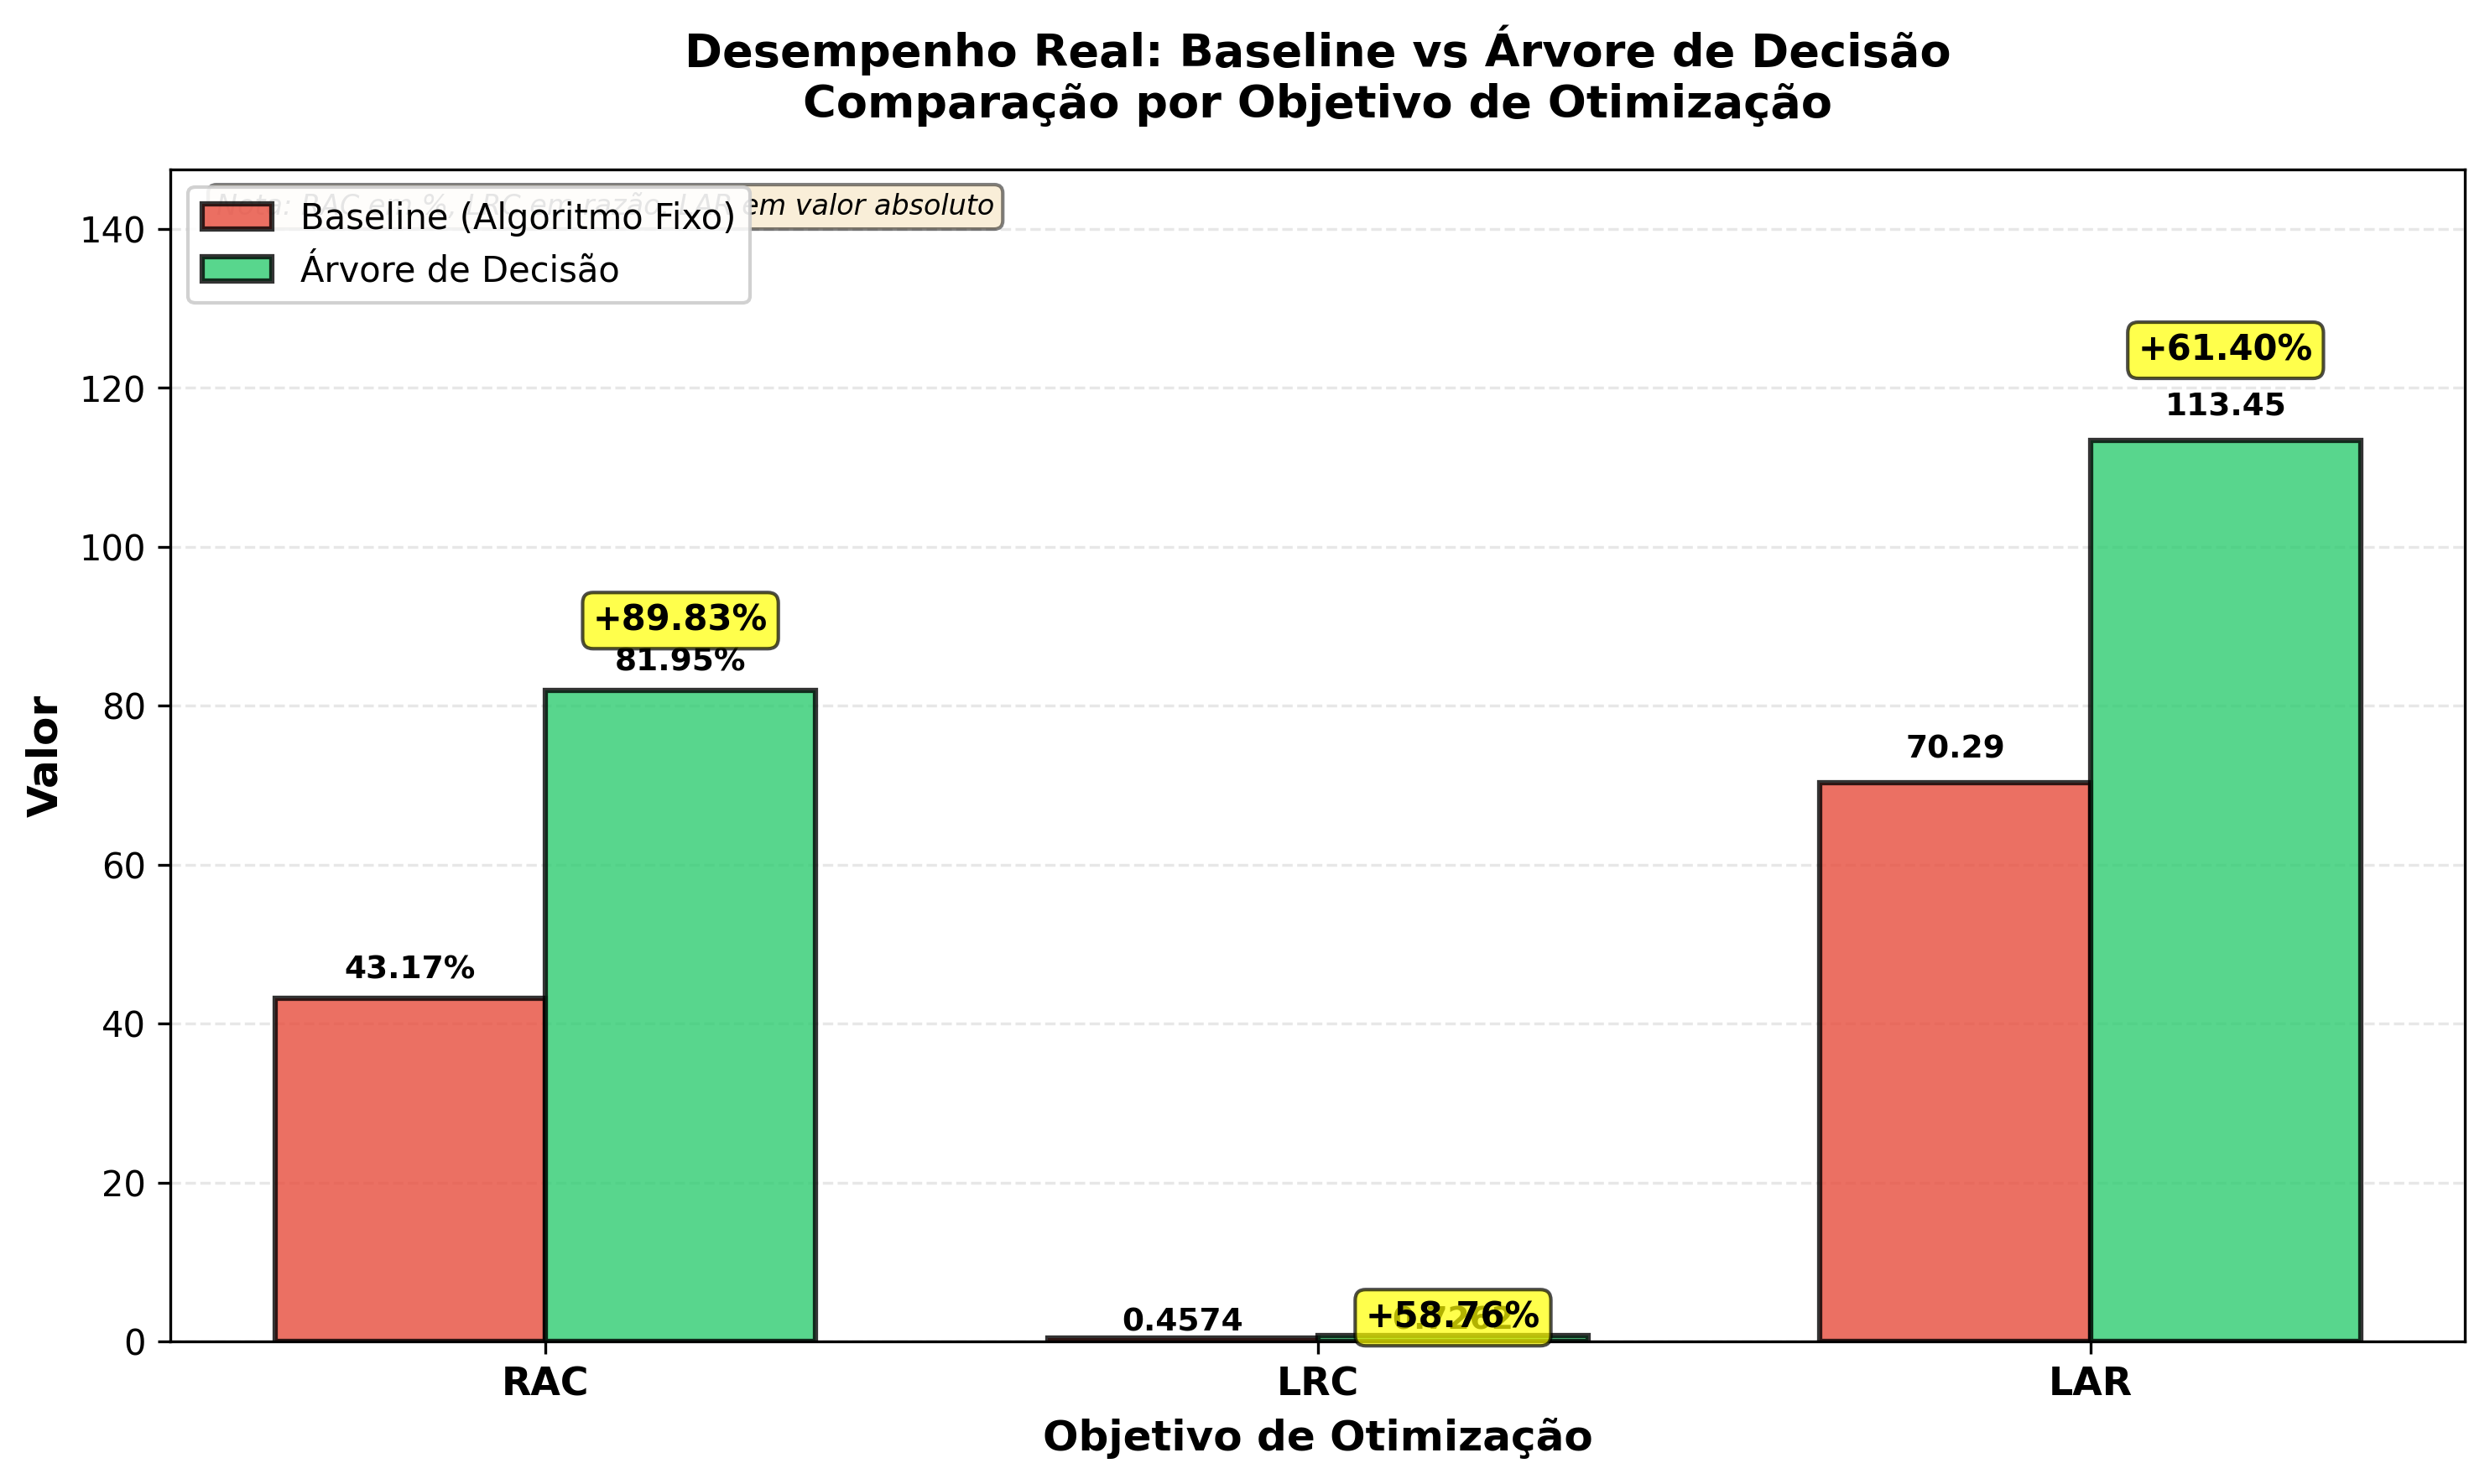
\includegraphics[width=0.95\textwidth]{real_performance_chart}
\caption{Real Operational Performance: Decision-Tree Selection vs Fixed-Algorithm Baseline, by Optimization Objective. Unlike Figure~\ref{fig:baseline-comparison}, which measures classification accuracy, this figure measures the actual RAC/LRC/LAR values achieved when each policy is used to serve the VNRs. Source: authors' own experimental results.}
\label{fig:real-performance-improvement}
\end{figure}

Results show that contextual selection via decision trees produces \textbf{substantial improvements in real operational performance} across all three objectives:

\begin{itemize}
    \item \textbf{RAC}: Acceptance rate increases from 43.17\% (fixed baseline) to 81.95\% (contextual selection), an absolute gain of +38.78 percentage points, i.e., \textbf{+89.83\%} relative improvement.
    \item \textbf{LRC}: Revenue-cost ratio increases from 0.4574 to 0.7262, an improvement of \textbf{+58.76\%}.
    \item \textbf{LAR}: Average revenue increases from 70.29 to 113.45 per VNR, an improvement of \textbf{+61.40\%}.
\end{itemize}

These results indicate that contextual selection via decision trees is significantly superior to using a fixed algorithm, with substantial improvements in all three evaluated objectives, and that the gains observed in classification accuracy (Figure~\ref{fig:baseline-comparison}) do translate into real operational gains (Figure~\ref{fig:real-performance-improvement}), even though the two are measured on different scales and should not be conflated.

The analysis reveals three additional patterns, discussed below.

\textcolor{red}{feio esse formato}

\textcolor{red}{[R: nao ha dado a consultar --- e questao de estrutura, e a critica procede. Os tres \texttt{subsubsection} seguintes tem de uma a tres frases cada, o que os enquadra nas diretrizes \#11 (paragrafo de uma frase) e \#26 (topicos). Ha ainda repeticao: o conteudo reproduz a Tabela~\ref{tab:algorithm-summary} e o argumento ja apresentado na Secao~\ref{subsec:discussion}. Sugestao: fundir os tres em um unico paragrafo corrido de analise, ou desloca-los para a discussao. Atencao adicional: os numeros citados nesses paragrafos vem da tabela sintetica --- ver anotacao junto a Tabela~\ref{tab:algorithm-summary}.]}

\subsubsection{No Algorithm is Universally Optimal}
As shown in Table~\ref{tab:algorithm-summary}, MIP maximizes acceptance rate (36.8\%), GA\_META maximizes revenue (400.6), D\_ROUND offers the best revenue-cost ratio (246.0), and PSO\_META is the fastest (0.309\,s). Each algorithm excels in a different dimension, and none dominates the others across all four metrics.

\subsubsection{Explicit Trade-offs}
MIP offers high acceptance but with elevated processing time (1.026\,s). D\_ROUND is very fast but with reduced acceptance (20.4\%). GA\_META offers a balanced trade-off between revenue and processing time.

\subsubsection{Justification for the Multi-Objective Approach}
This performance variation empirically evidences that:
\begin{itemize}
    \item A single fixed algorithm cannot serve all operational contexts well.
    \item Contextual selection based on network state and VNR characteristics is essential.
    \item Multi-objective decision trees learn to map context $\rightarrow$ appropriate algorithm for a chosen objective.
    \item The system can adapt priorities at runtime (acceptance vs.\ revenue vs.\ processing time) without retraining.
\end{itemize}

\begin{table}[htbp]
\centering
\caption{F1-Score per Class - RAC Objective (Balanced Models)}
\label{tab:f1-per-class}
\begin{tabular}{lccc}
\toprule
\textbf{Algorithm} & \textbf{Precision} & \textbf{Recall} & \textbf{F1-Score} \\
\midrule
GA\_Meta & 0.73 & 0.74 & 0.73 \\
MCTS & 0.78 & 0.72 & 0.75 \\
PL\_Rank & 0.77 & 0.66 & 0.71 \\
D\_Round & 0.61 & 0.59 & 0.60 \\
MIP & 0.49 & 0.57 & 0.53 \\
SA\_Meta & 0.43 & 0.56 & 0.49 \\
RW\_Rank\_BFS & 0.67 & 0.25 & 0.36 \\
PSO\_Meta & 0.22 & 0.67 & 0.33 \\
\midrule
\textbf{F1-Macro} & \multicolumn{3}{c}{\textbf{0.56}} \\
\textbf{F1-Weighted} & \multicolumn{3}{c}{\textbf{0.68}} \\
\bottomrule
\end{tabular}
\end{table}

The detailed analysis presented in Table~\ref{tab:f1-per-class} reveals that balancing techniques allow capturing patterns even from minority classes. Algorithms such as GA\_Meta, MCTS, and PL\_Rank present F1-Score above 0.70, indicating good prediction capability. Minority classes such as PSO\_Meta and RW\_Rank\_BFS present lower F1-Score (0.33 and 0.36, respectively), but still well above zero, demonstrating that the model can identify patterns even for these under-represented classes. F1-Macro of 0.56 and F1-Weighted of 0.68 indicate that the model presents reasonably balanced performance across classes, with better performance on more frequent classes, as expected.

\subsection{Interpretability Analysis}

One of the main advantages of the approach is that each decision can be traced through the decision tree. Figure~\ref{fig:decision-tree-example} shows a simplified fragment of the trained RAC tree, illustrating how the model classifies VNRs:

\begin{figure}[htbp]
    \centering
    
\includegraphics[width=0.8\textwidth]{tree_visualization_example}
    \caption{Simplified fragment of the trained RAC decision tree, showing the topmost splits used to route a VNR toward an algorithm recommendation. Source: authors' own trained model.}
    \label{fig:decision-tree-example}
\end{figure}

Unlike deep neural networks (black box), operators can understand \textbf{exactly why} an algorithm was selected. For example, the extracted rule shown in Figure~\ref{fig:tree-example-path} can be read as:

\textit{``If VNR size is below 30\% of the physical network AND node utilization exceeds 70\%, then select MIP (an exact algorithm, more likely to find a feasible solution under congestion). Otherwise, if connectivity exceeds 0.5, select GA-Meta.''}

Additionally, \textit{feature} importance analysis reveals which characteristics are most relevant for each objective. \textcolor{red}{explicar as features} \textcolor{red}{[R: alem de faltar a explicacao, ha um descasamento entre o texto e o codigo que precisa ser resolvido antes de escreve-la.
\textbf{(a) O numero 27 nao existe no codigo.} As listas canonicas de \emph{features} sao de 25 (\texttt{3\_train\_decision\_trees\_balanced.py:27-64}), 35 (\texttt{3\_train\_decision\_trees\_enhanced.py:34-87}) e \textbf{34} (\emph{per-topology}, \texttt{3\_train\_decision\_trees\_optimized.py:188}); os proprios \texttt{.pkl} registram \texttt{n\_features\_in\_} = 25, 34, 35, 19, 32 ou 60 --- nunca 27. As Figuras~\ref{fig:feature-importance-rac}--\ref{fig:feature-importance-lar} vem do modelo de \textbf{34}.
\textbf{(b) A conta 9+4+3+10+1 exclui as 8 \emph{features} \emph{engineered}} --- entre elas \texttt{resource\_efficiency}, que este mesmo paragrafo aponta como a mais importante (0,134). O artigo, portanto, contradiz a si proprio: descreve um conjunto que nao contem a variavel que declara dominante.
\textbf{(c) Nao existem indices de Gini como \emph{feature}.} A busca no repositorio retorna zero ocorrencias; as unicas mencoes a Gini sao o criterio de \emph{split} do scikit-learn e a ``Gini-importance'' das legendas. Tambem nao existem ``memory fragmentation'' nem ``topological diversity indices''. As tres \emph{proxies} de fragmentacao reais (\texttt{2b\_create\_enhanced\_datasets.py:34-49}) derivam de apenas dois escalares agregados (\texttt{p\_net\_node\_util}, \texttt{p\_net\_link\_util}), sem qualquer estatistica por no --- que e exatamente o que um indice de Gini exigiria. A descricao da Secao~\ref{sec:Proposal} precisa ser substituida pelas formulas reais.
\textbf{(d) Bug a corrigir antes de qualquer retreino:} a constante \texttt{10457} usada em \texttt{p\_net\_overall\_util} (\texttt{2\_prepare\_dataset.py:94}) e fixa para as tres topologias, mas os recursos iniciais diferem; o resultado assume valores \textbf{negativos} (faixa medida: $-0{,}65$ a $0{,}74$) para \texttt{fat\_tree} e \texttt{waxman\_16}, contaminando todas as \emph{features} derivadas dela.]}Feature importance here is computed as the mean decrease in Gini impurity attributable to each feature across all splits in the trained tree, averaged over the three topologies. For RAC (Request Acceptance Rate) and LRC (Long-Term Revenue-to-Cost), resource efficiency ($resource\_efficiency$) is the most critical \textit{feature}, with importance of 0.134 and 0.113 respectively. In the case of LAR (Long-Term Average Revenue), VNR link demand ($v\_net\_demand\_per\_link$) and total demand ($v\_net\_total\_demand$) are the dominant \textit{features}. These findings confirm that different objectives prioritize distinct characteristics of VNRs and physical network state. Figure~\ref{fig:feature-importance-rac} exemplifies \textit{feature} importance for the RAC objective, while Figures~\ref{fig:feature-importance-lrc} and~\ref{fig:feature-importance-lar} present results for the remaining objectives.

\begin{figure}[htbp]
    \centering
    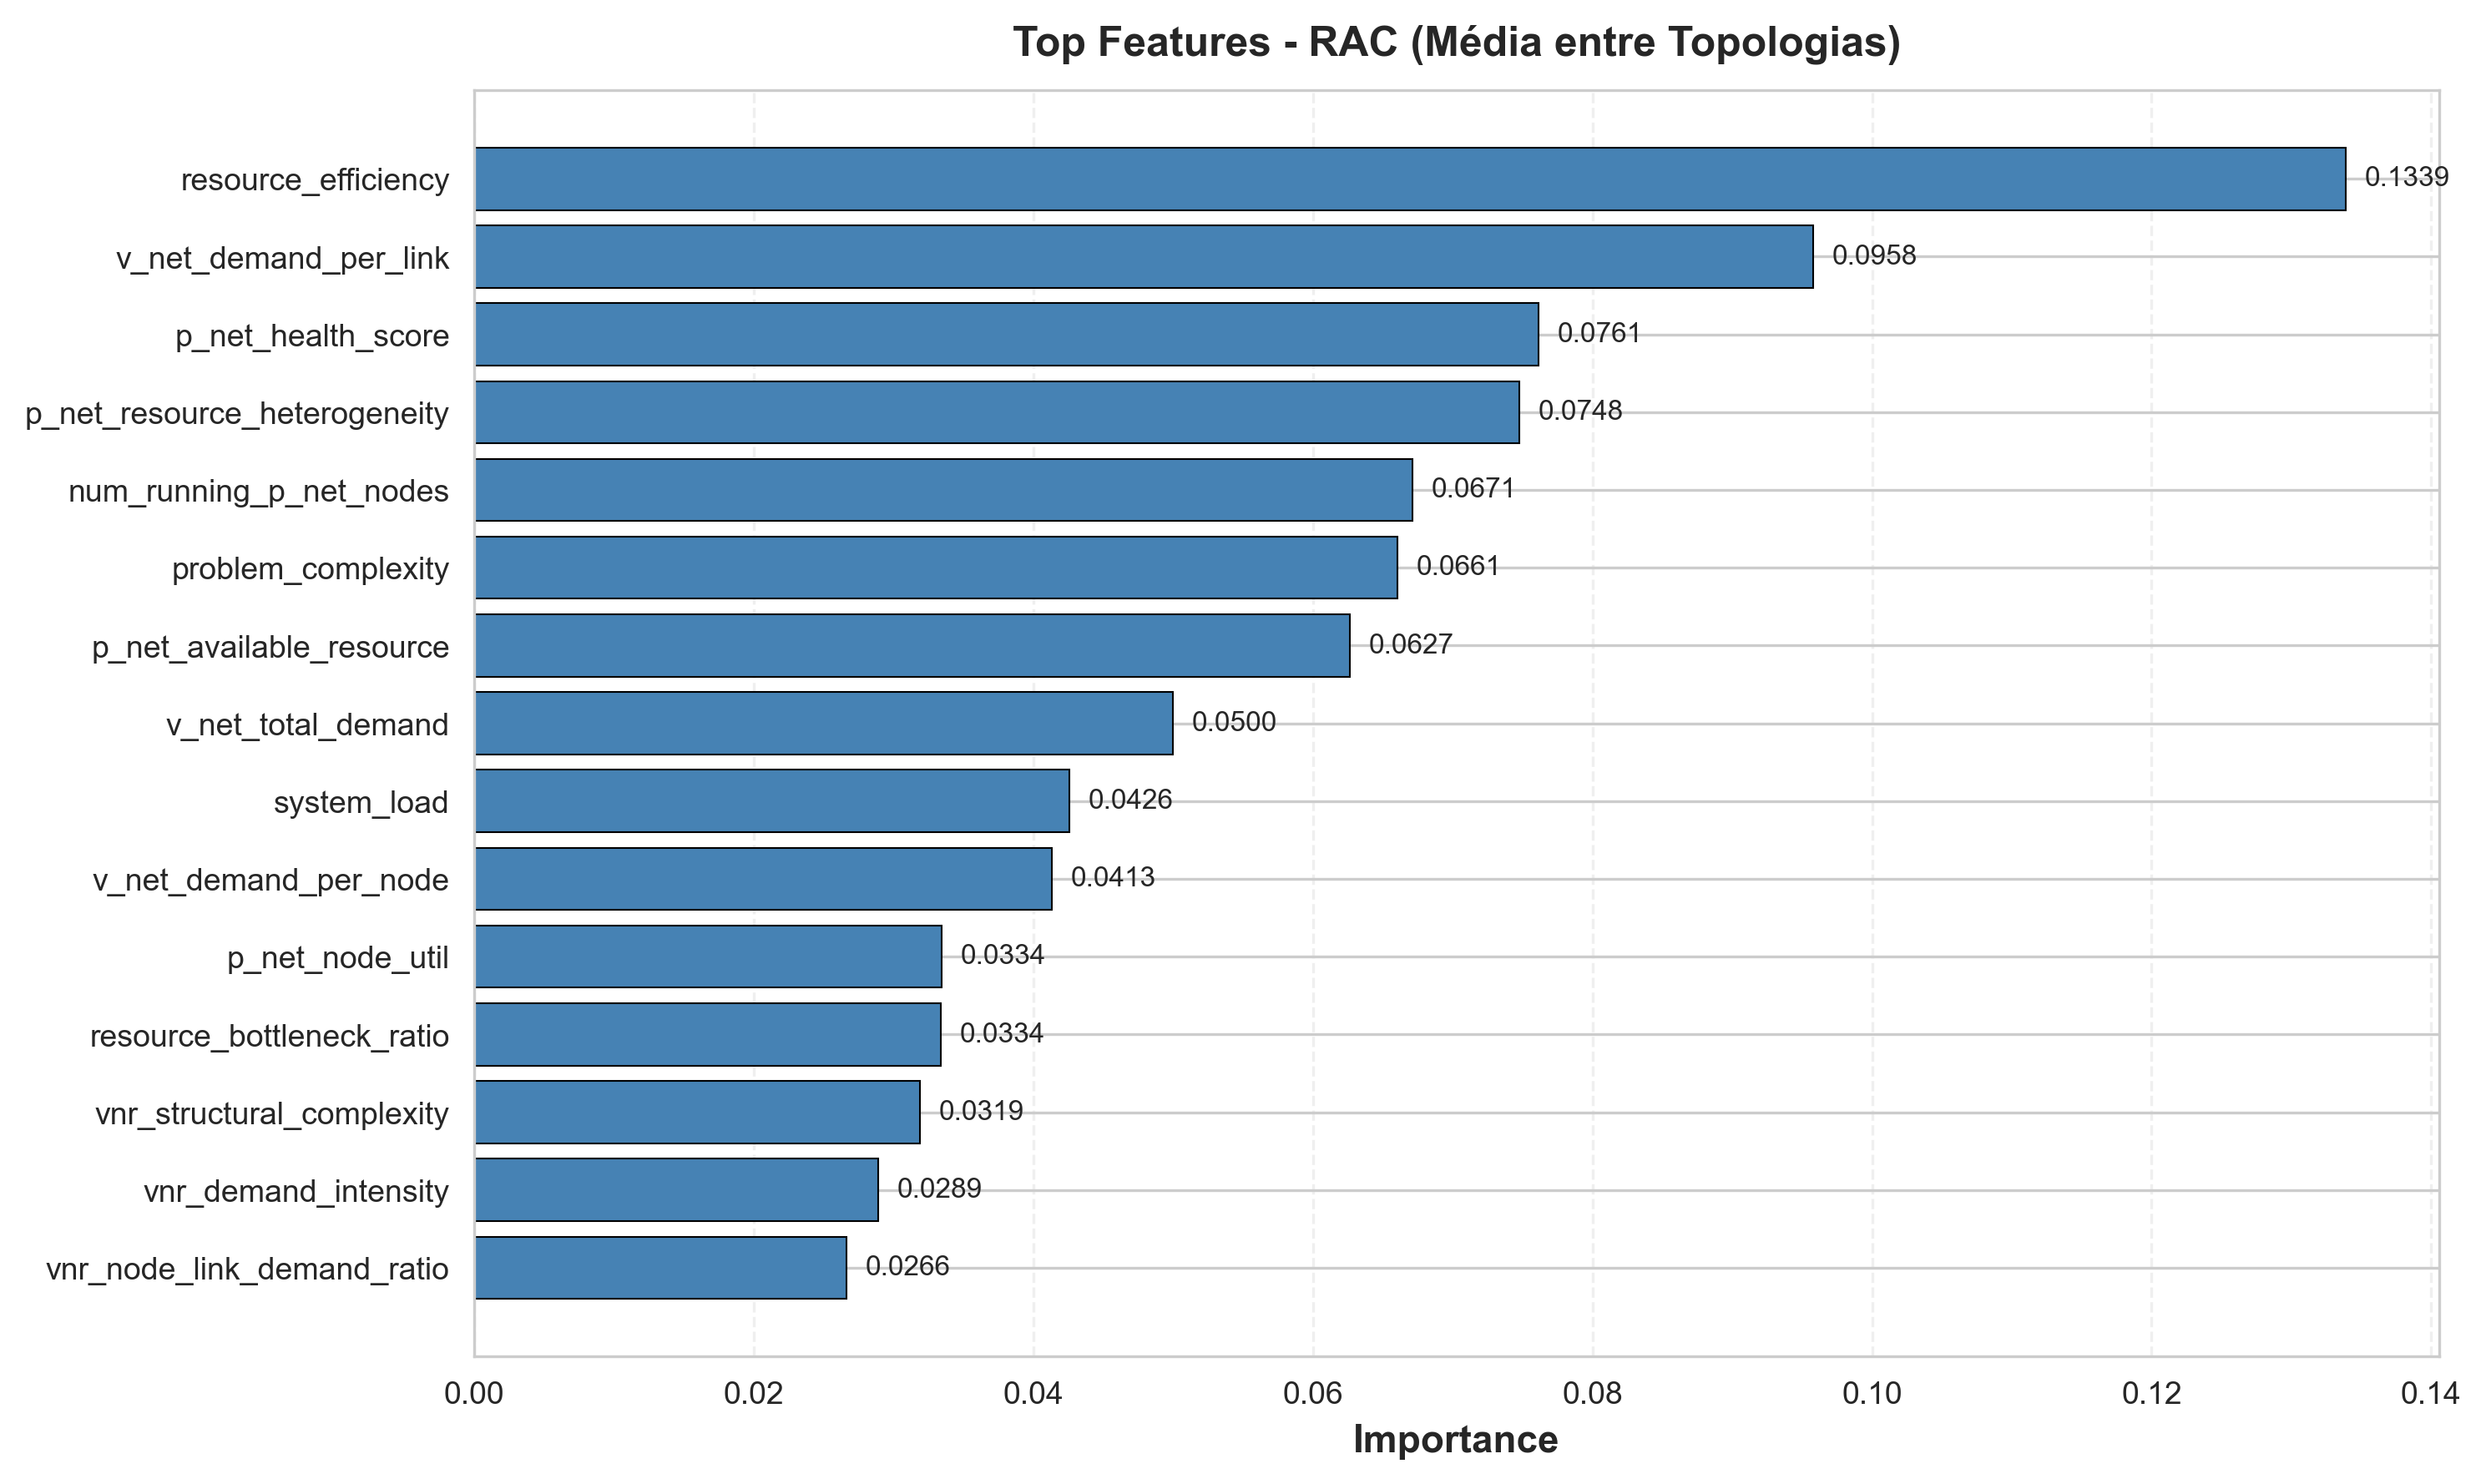
\includegraphics[width=0.95\textwidth]{per_objective_rac}
    \caption{Feature Importance for the RAC objective. Top 15 features by mean Gini-importance, averaged across the three topologies. Resource efficiency ($resource\_efficiency$) is the most critical feature (importance 0.134), followed by VNR link demand ($v\_net\_demand\_per\_link$, 0.096). Source: authors' own trained RAC model.}
    \label{fig:feature-importance-rac}
\end{figure}

\begin{figure}[htbp]
    \centering
    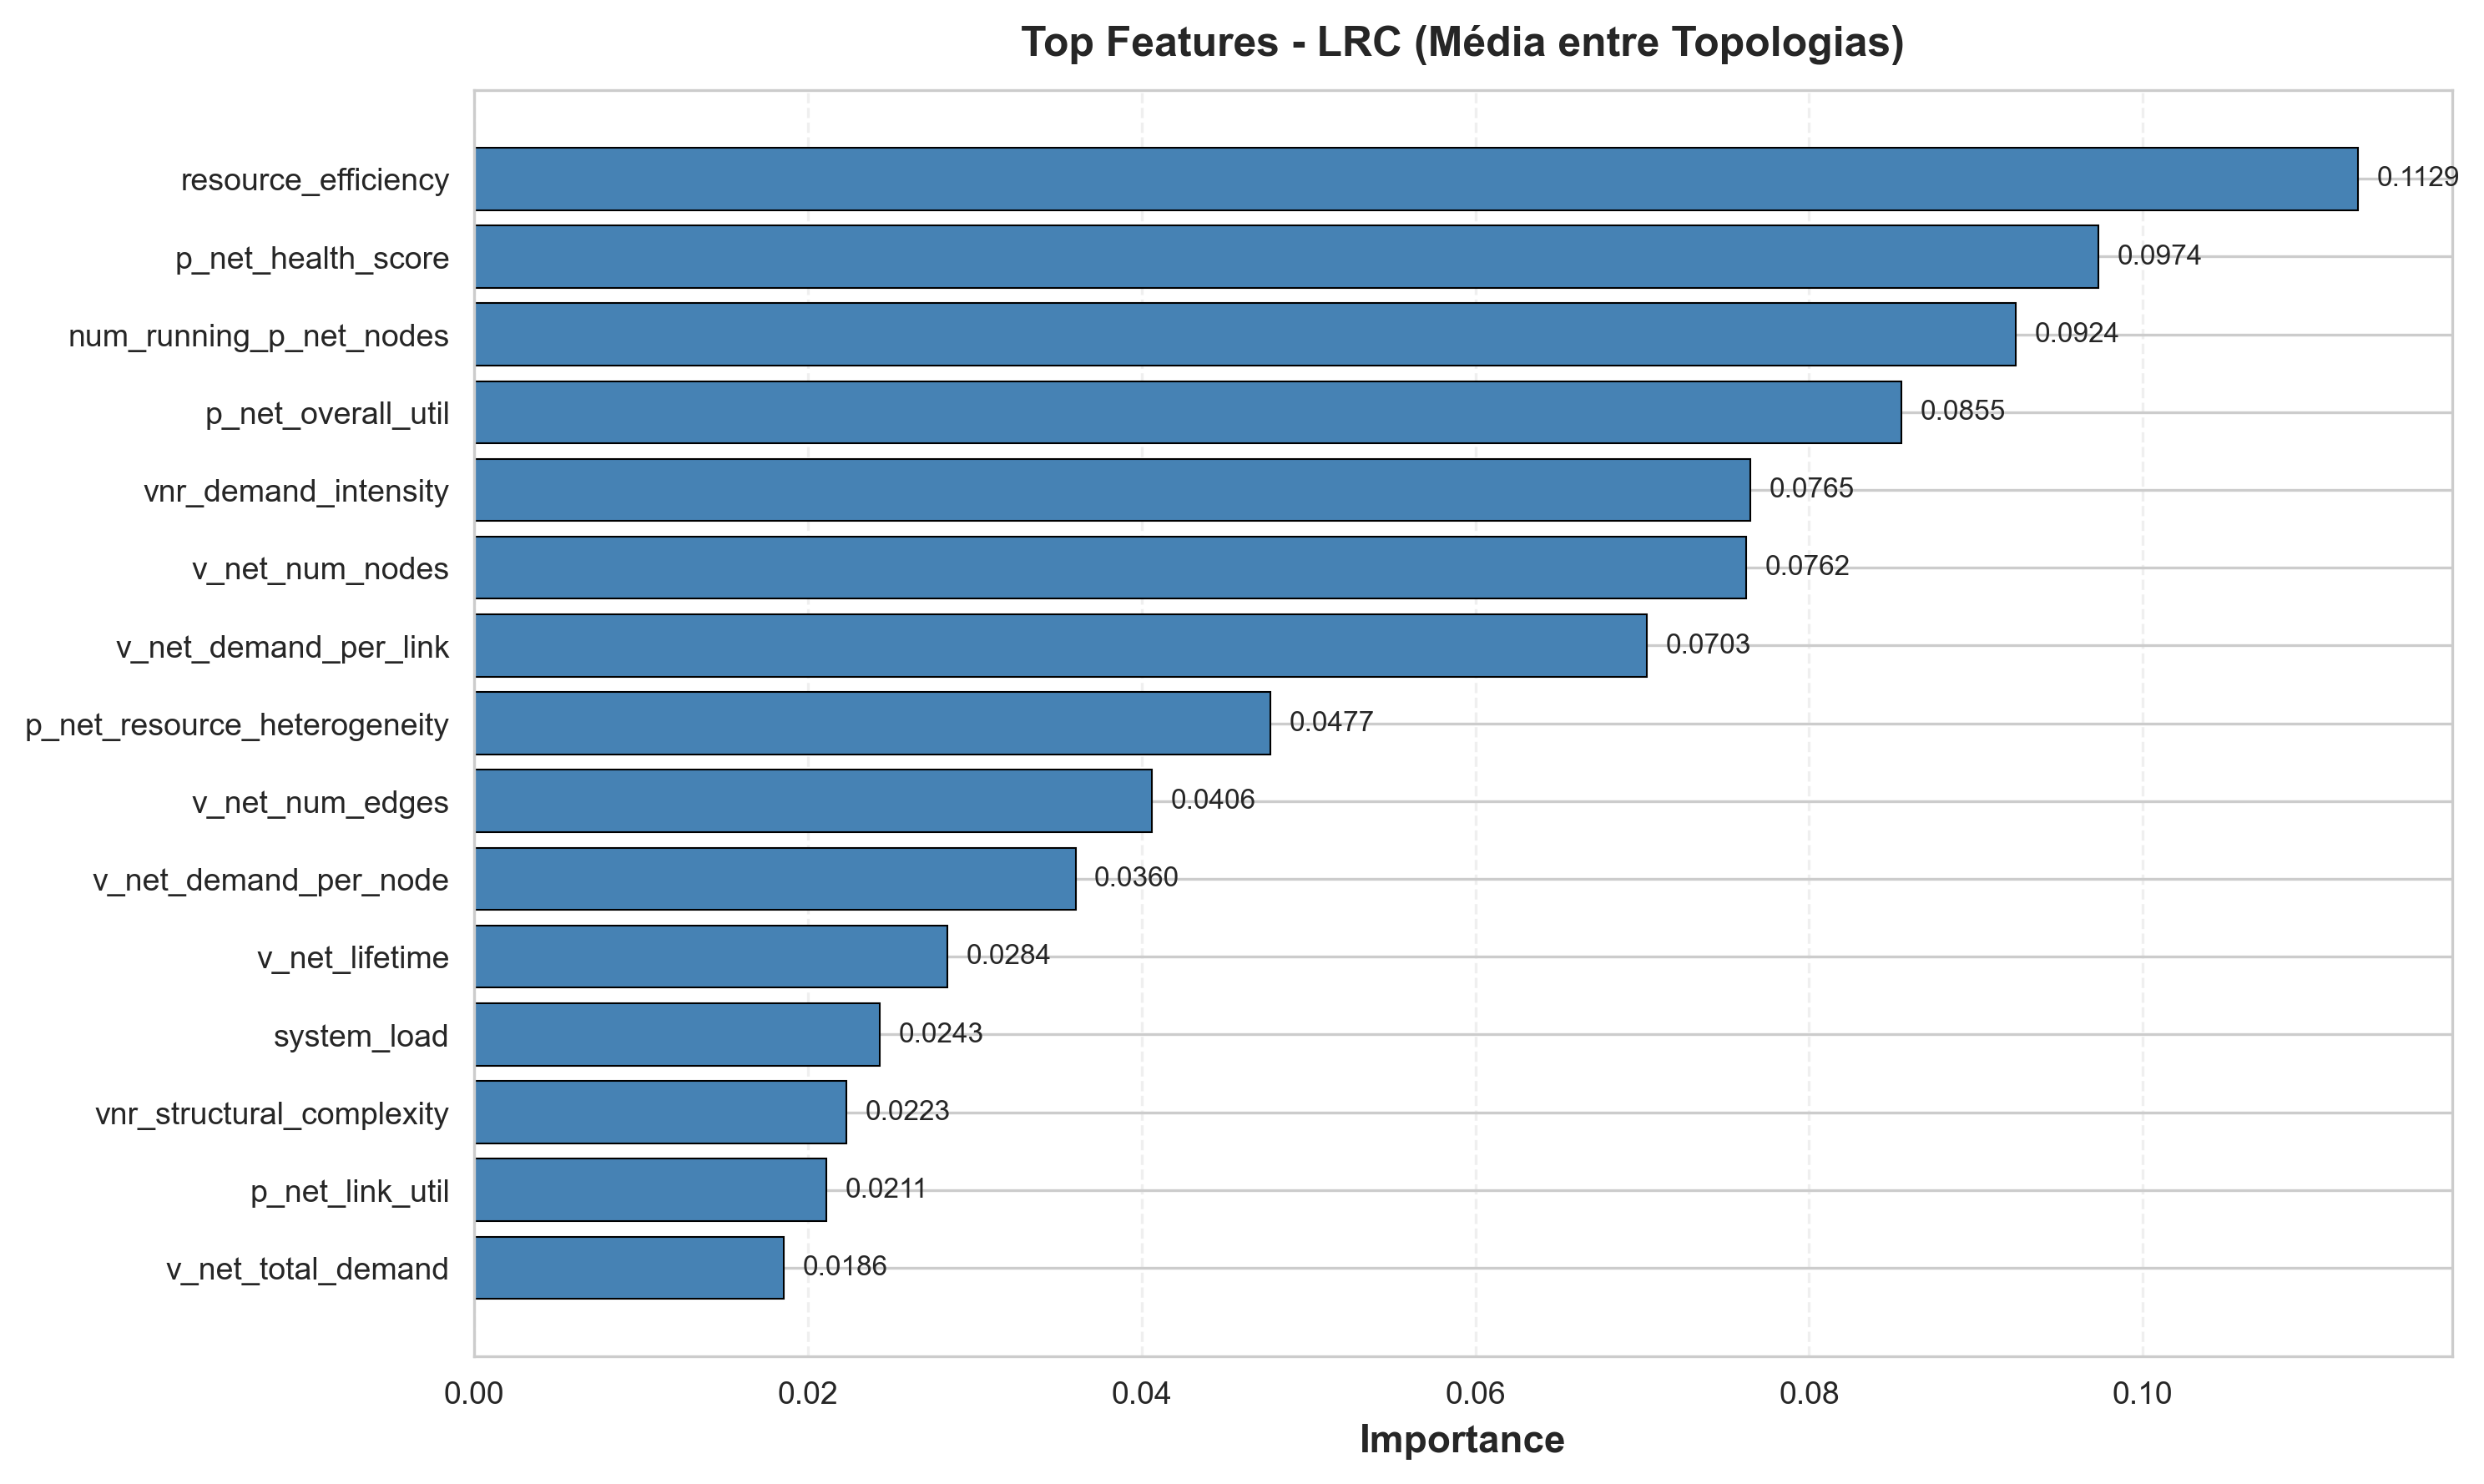
\includegraphics[width=0.95\textwidth]{per_objective_lrc}
    \caption{Feature Importance for the LRC objective. Top 15 features by mean Gini-importance, averaged across the three topologies. Resource efficiency ($resource\_efficiency$) is the most critical feature (importance 0.113), followed by physical network health score ($p\_net\_health\_score$, 0.097). Source: authors' own trained LRC model.}
    \label{fig:feature-importance-lrc}
\end{figure}

\begin{figure}[htbp]
    \centering
    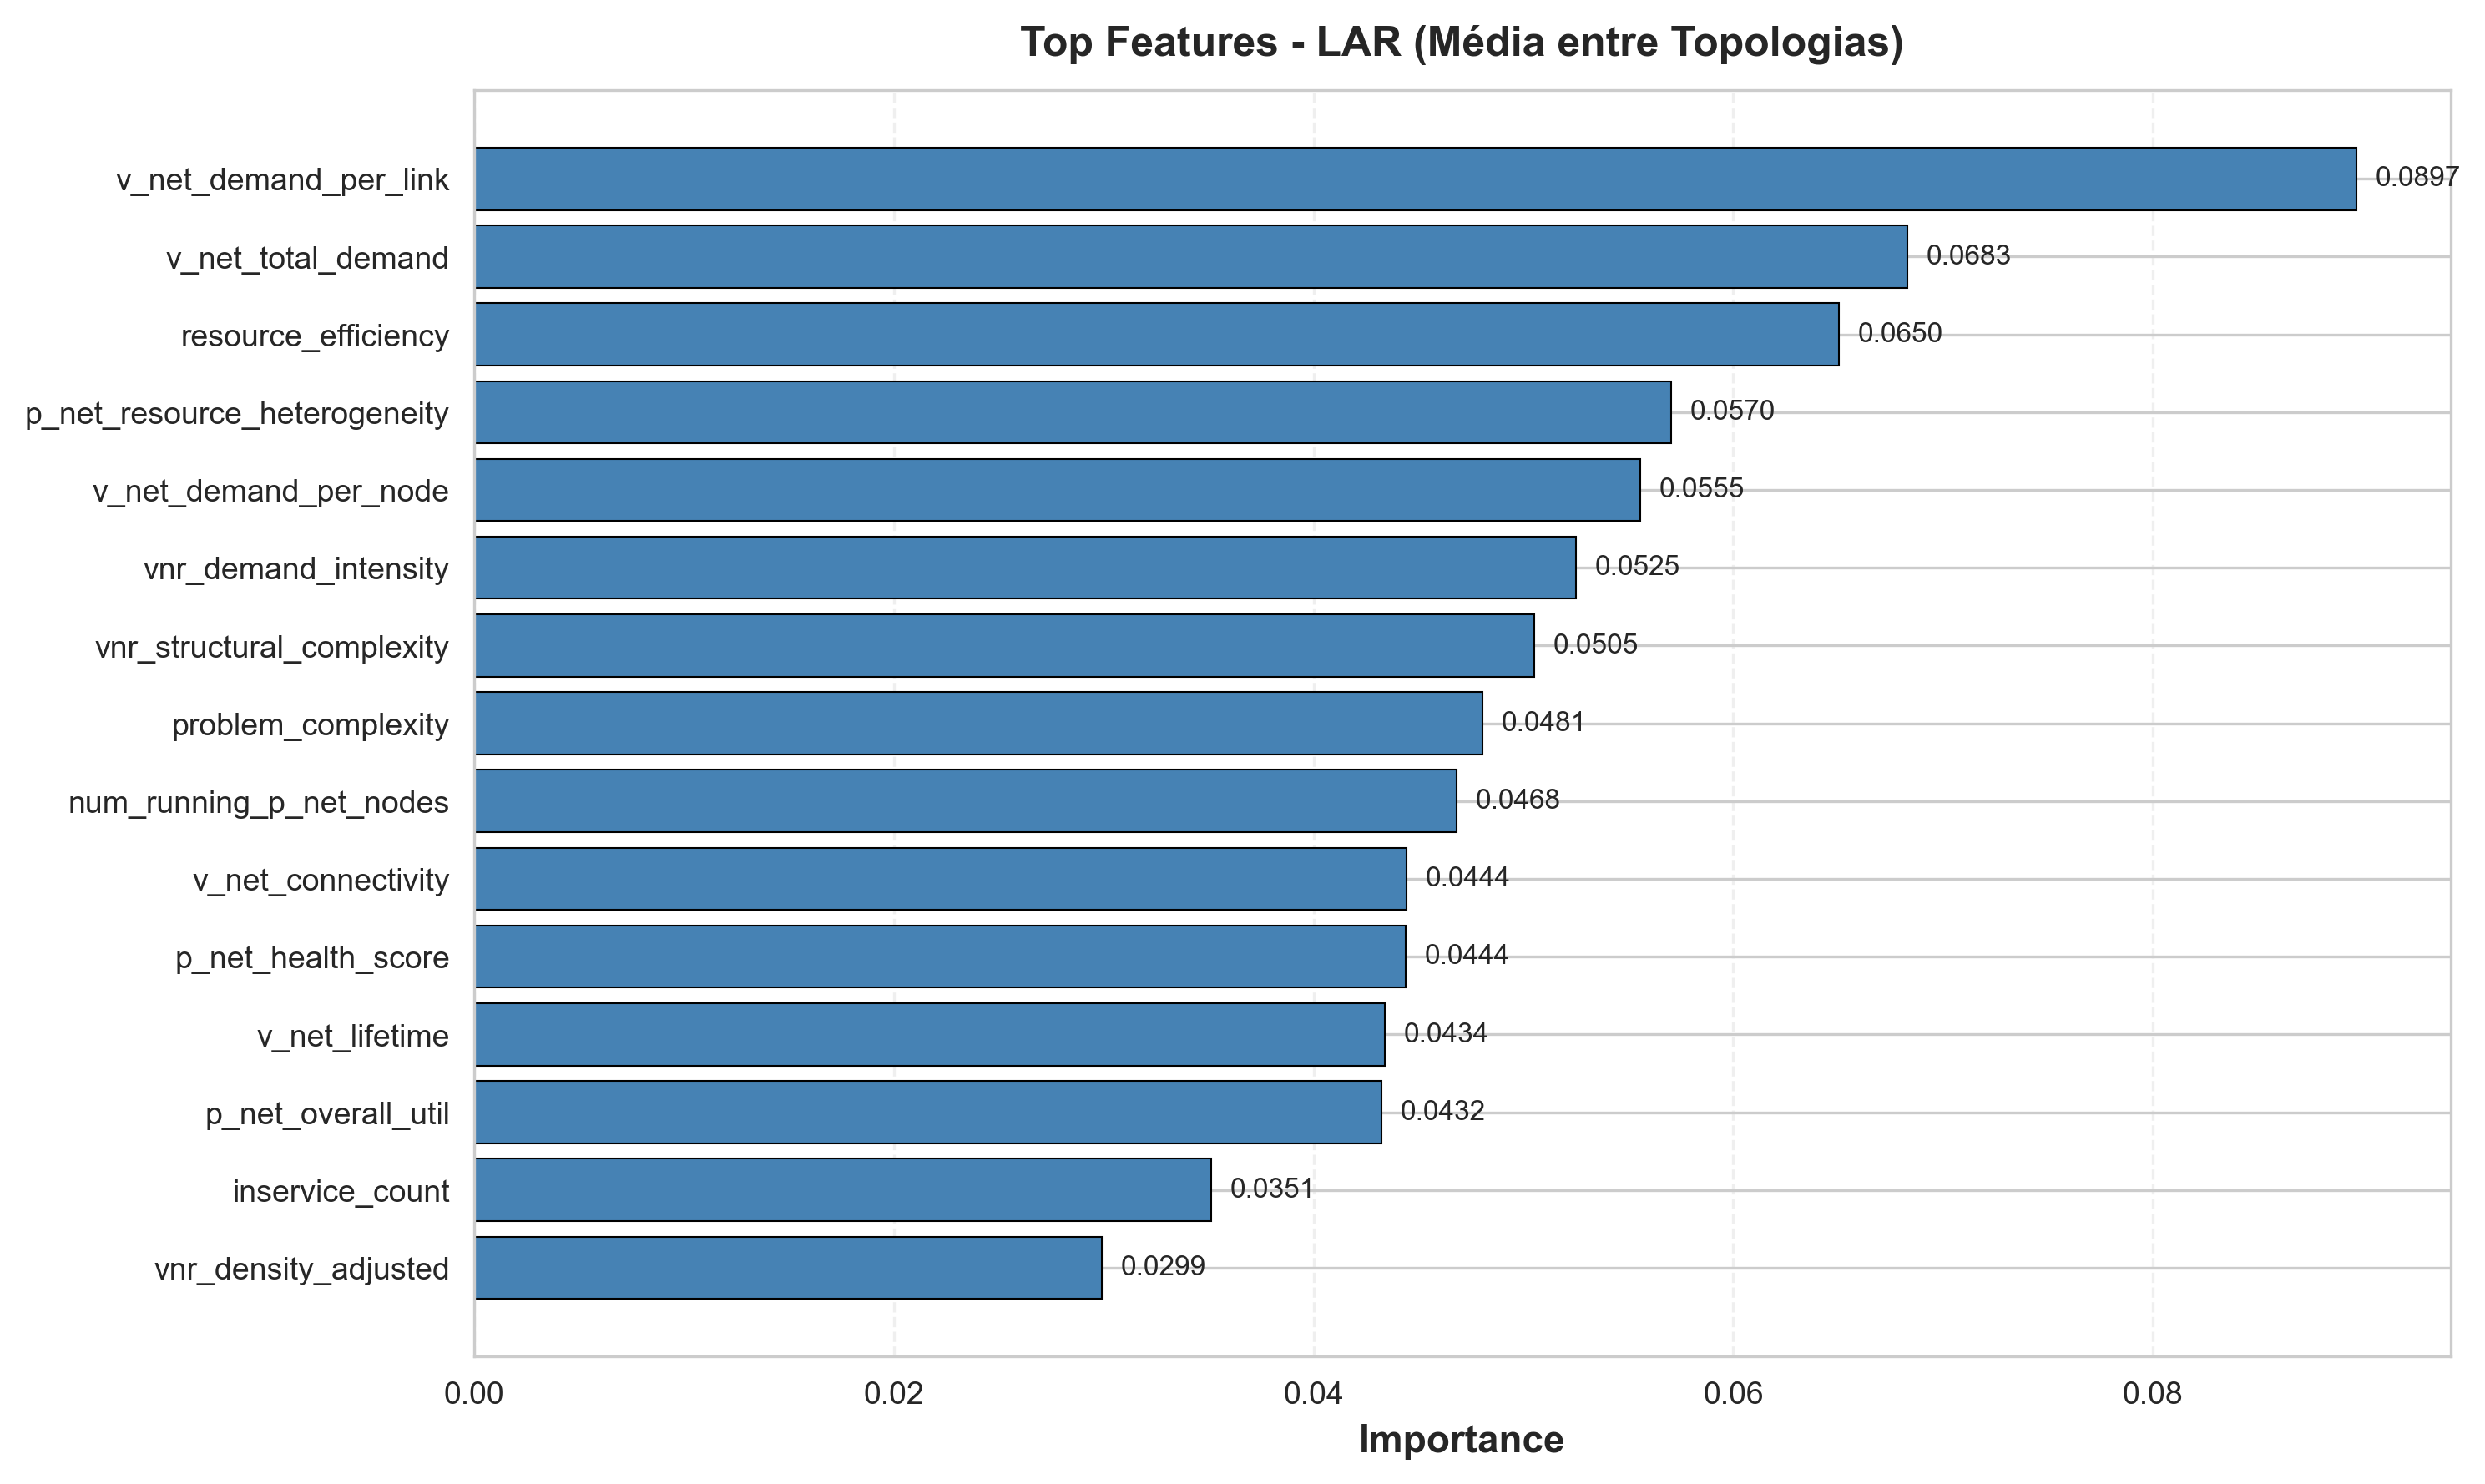
\includegraphics[width=0.95\textwidth]{per_objective_lar}
    \caption{Feature Importance for the LAR objective. Top 15 features by mean Gini-importance, averaged across the three topologies. VNR link demand ($v\_net\_demand\_per\_link$) is the most important feature (importance 0.090), followed by total demand ($v\_net\_total\_demand$, 0.068). Source: authors' own trained LAR model.}
    \label{fig:feature-importance-lar}
\end{figure}

This interpretability is critical, as it allows regulators to perform audits by verifying decisions made by the system, facilitates debugging work by enabling operators to understand system behavior, and increases confidence and acceptance of \textit{zero-touch} automation.

\subsection{Inference Latency}

Prediction latency measurements for each model (based on a benchmark with 8,000 iterations, executed on the same hardware used for training):

\begin{itemize}
    \item \textbf{Average time}: 0.034\,ms per prediction
    \item \textbf{Percentile p99}: 0.055\,ms (worst case: 0.119\,ms)
    \item \textbf{RL Comparison}: FlagVNE requires 50--200\,ms per decision~\cite{ijcai-2024-flagvne}
\end{itemize}

Figure~\ref{fig:inference-latency-cdf} presents the cumulative distribution function (CDF) of inference latency, comparing the proposed approach with the latency range reported for FlagVNE~\cite{ijcai-2024-flagvne}. The results show that more than 99\% of predictions are performed in less than 0.06\,ms, demonstrating consistency in sub-millisecond latency.

\begin{figure}[htbp]
\centering
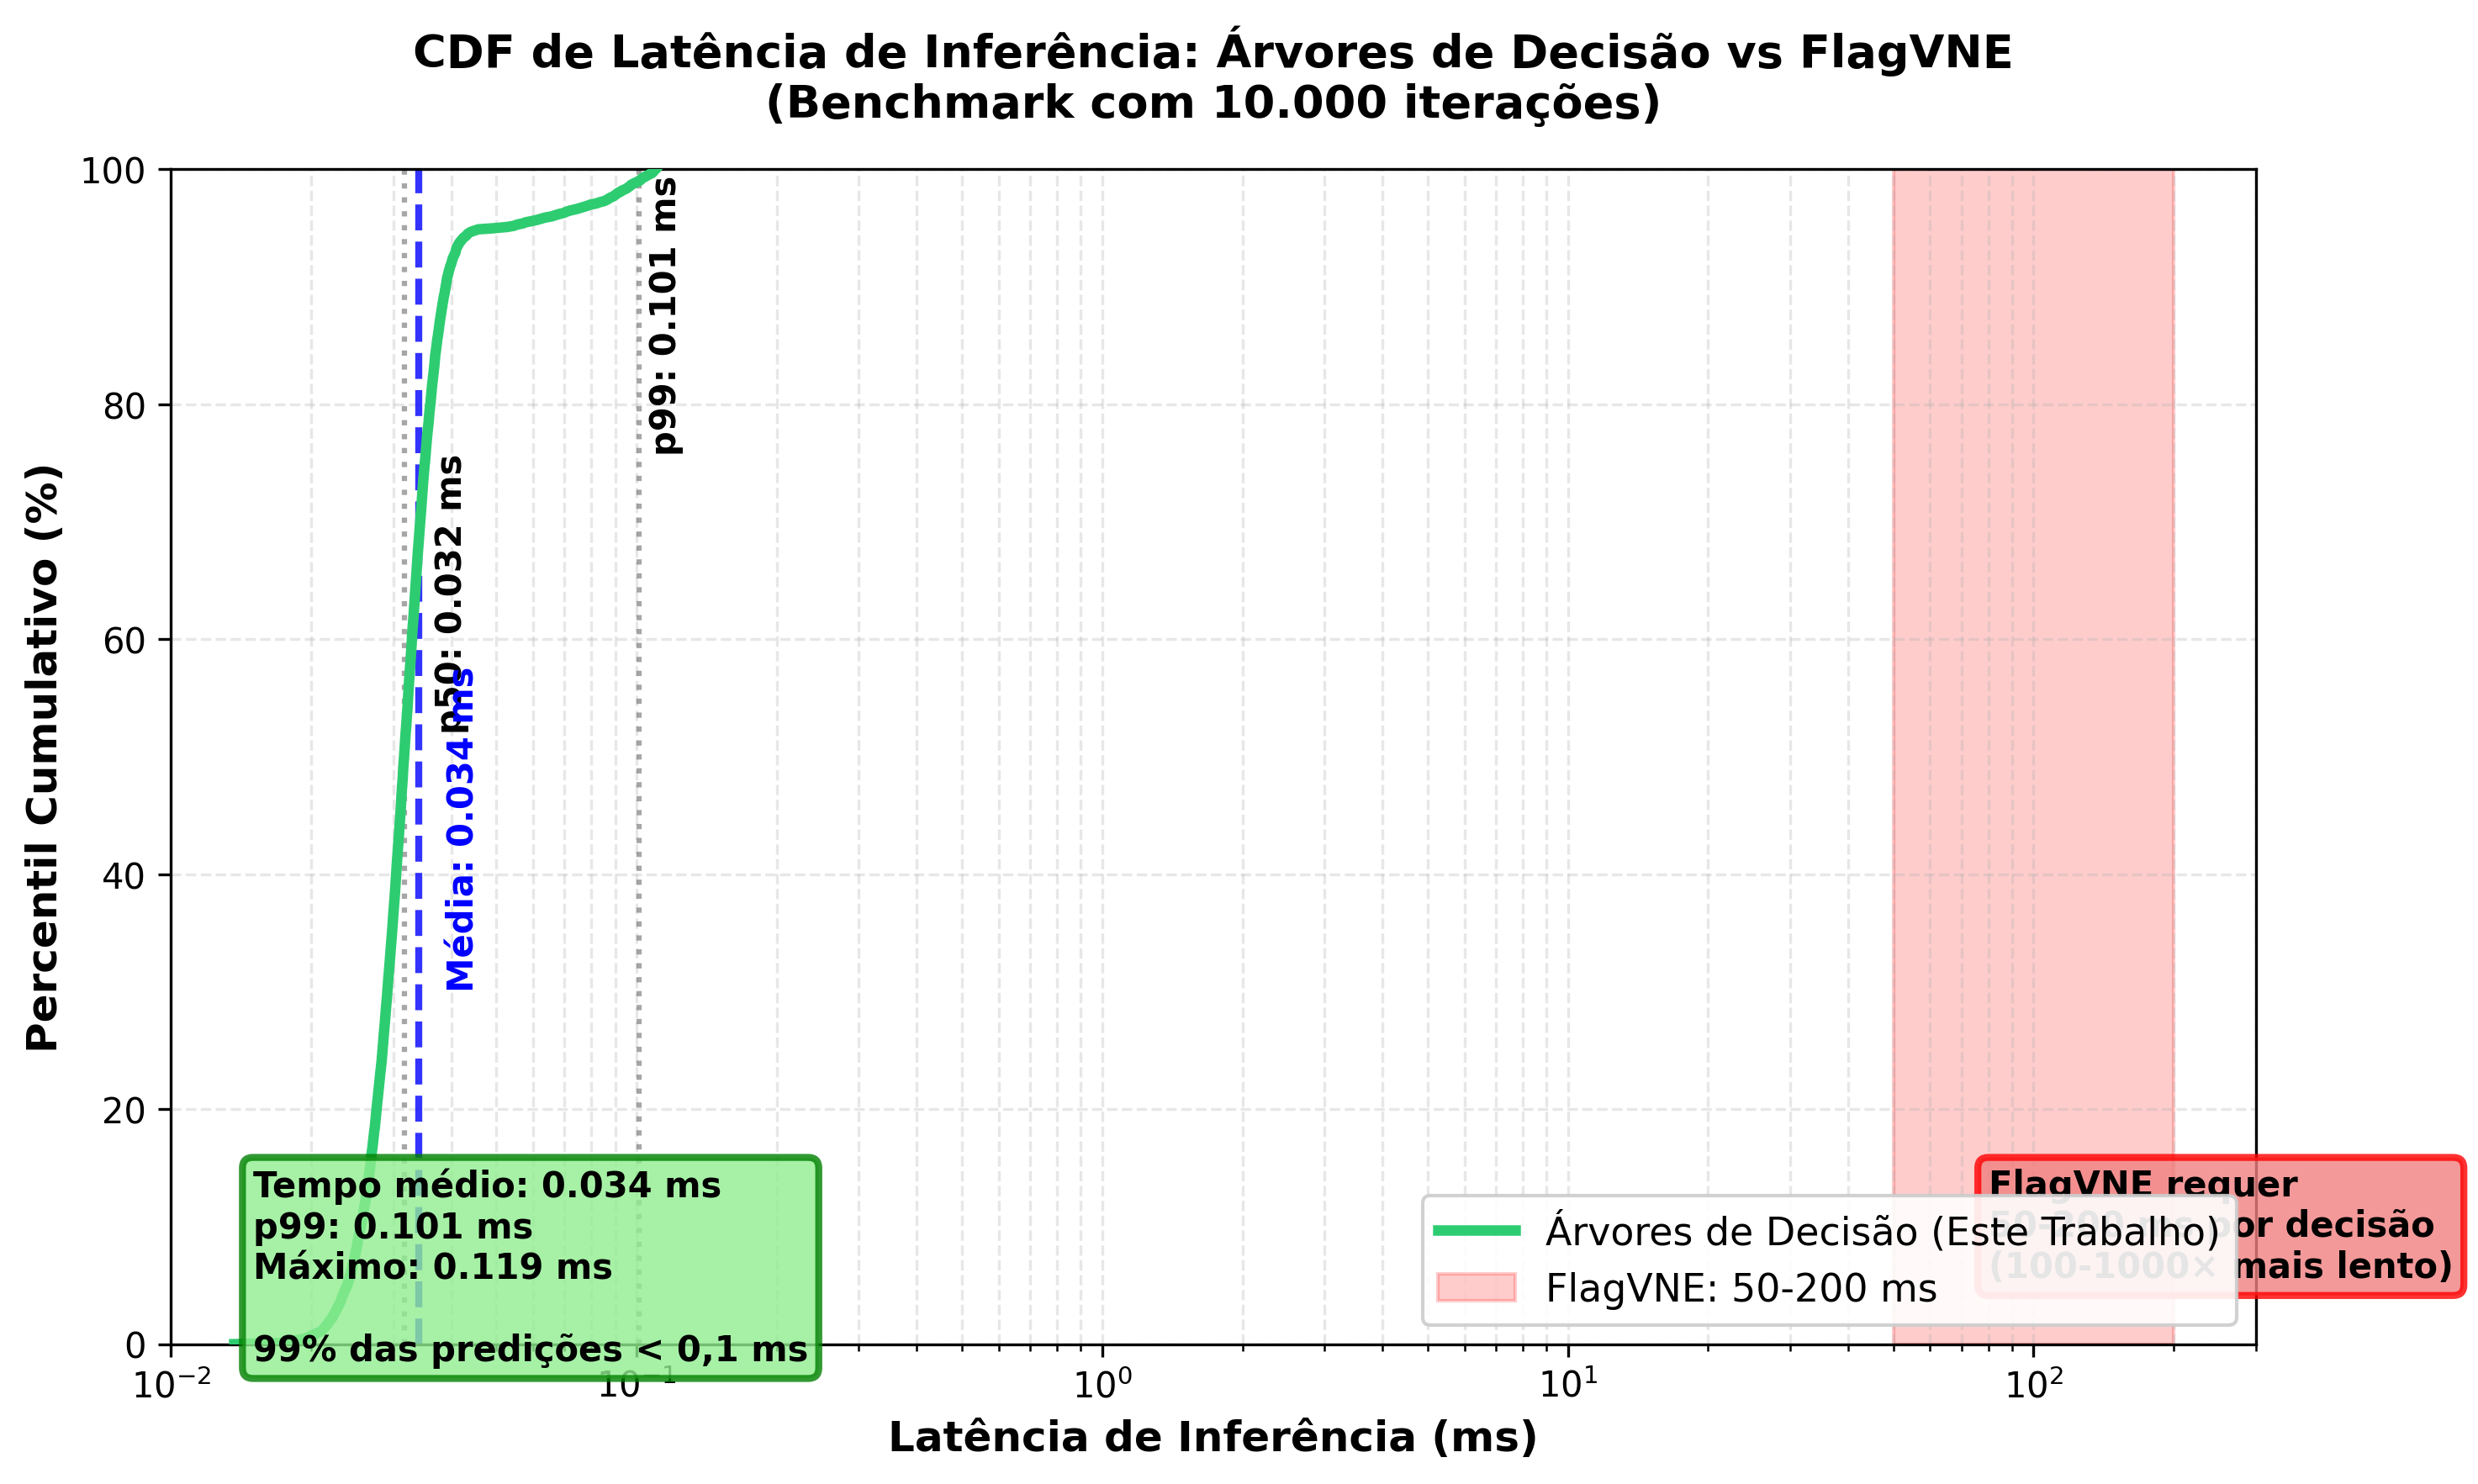
\includegraphics[width=0.95\textwidth]{inference_latency_cdf}
\caption{Inference Latency CDF: Decision Trees (authors' own benchmark) vs FlagVNE (latency range as reported in~\cite{ijcai-2024-flagvne}). The proposed approach presents latency consistently below 0.1\,ms, while FlagVNE requires 50--200\,ms per decision; note the different scale used for the FlagVNE range on the secondary axis.}
\label{fig:inference-latency-cdf}
\end{figure}

Sub-millisecond latency enables \textit{online} real-time decision making, critical for \textit{zero-touch} operation.

\section{Conclusion}
\label{sec:Conclusion}

This work proposed an approach for \textit{zero-touch} selection of \textit{Virtual Network Embedding} algorithms using multi-objective decision trees, considering virtual network request characteristics and physical infrastructure state.
The approach differentiates itself from deep-learning alternatives by offering complete interpretability through explicit decision paths and inference latency below 1\,ms, allowing real-time \textit{online} operation.

Specifically, experimental results show that the foundations of the proposed approach (decision trees, multi-objective optimization, and interpretability) are potential candidates to achieve \textit{zero-touch} network control according to the ETSI ZSM standard.
The experimental analysis, based on three \textit{datacenter} topologies (Tree, Fat-Tree, and Waxman-16) with 8,000 virtual network requests, showed that contextual algorithm selection can reduce processing time and improve acceptance rate in various scenarios, without requiring software updates at infrastructure endpoints.

The results show that the proposed approach, operating in conjunction with traditional VNE algorithms such as MIP, GA-Meta, and PL-Rank, can significantly improve operational performance:
\begin{itemize}
    \item \textbf{Acceptance Rate Improvement}: +38.78 percentage points compared to the fixed-algorithm \textit{baseline} (from 43.17\% to 81.95\%, \textbf{+89.83\%} relative)
    \item \textbf{Top-3 Accuracy}: Between 79.1\% and 85.9\%, showing robustness in predicting the best algorithm
    \item \textbf{Revenue-Cost Ratio Improvement}: +58.76\% (from 0.4574 to 0.7262)
    \item \textbf{Average Revenue Improvement}: +61.40\% (from 70.29 to 113.45 per VNR)
\end{itemize}

The class balancing techniques used (custom weights $1/\sqrt{f}$ and hyperparameter tuning) were essential to capture the patterns of minority classes, resulting in an F1-Macro of 0.56 for the RAC objective.
Additionally, experimental results empirically confirmed that no VNE algorithm is universally optimal, validating the need for contextual selection based on request characteristics and network state.

As limitations, the model was trained on three simulated topologies, and the characteristics capture instantaneous network state; results have not yet been validated with statistical significance testing (e.g., confidence intervals across the ten random seeds) or on production traffic traces. \textcolor{red}{[R: a lista de limitacoes esta incompleta frente ao que o codigo revela. Faltam, no minimo: (i) a avaliacao de desempenho real cobre 410 VNRs de \textbf{duas} topologias, nao as tres declaradas; (ii) e \emph{replay} tabular \emph{offline}, sem re-simulacao, logo nao captura o efeito das escolhas sobre o estado futuro da rede; (iii) a rotulagem compara algoritmos executados em estados divergentes da rede fisica. Sobre este ultimo ponto, o experimento \texttt{ccis/} do proprio repositorio --- que avalia todos os candidatos sobre o mesmo estado --- obtem arvore 47,0\% contra melhor fixo 49,3\% (\texttt{ccis/results/tree\_summary.json}), resultado oposto ao reportado aqui. Essa divergencia precisa ser resolvida ou declarada antes da submissao.]}
As future work, promising directions include \textit{transfer learning} between topologies, incorporation of temporal history of requests, statistically-grounded evaluation across seeds, and validation in production environments with real \textit{datacenter} workloads.

%===================================================================

\bibliographystyle{splncs04}
\bibliography{references}

\end{document}